\section{Systematic uncertainties}
\label{sec:uncertainties}

The background and signal predictions are affected by systematic uncertainties that have to be estimated and taken into account in the signal extraction procedure. This section includes a list of the relevant systematic uncertainties for this analysis and how they are estimated.% Most of the systematic uncertainties are dedicated to samples that are not normalized on data or the shape is taken from simulation.


\subsection{Uncertainties affecting the data-driven main background estimation}

\subsubsection{Normalization}

The predictiond of the normalization and shape of main background, \V + jets, are both taken from data. The normalization is extracted from fits to the jet mass sidebands with arbitrary functions tested on simulation. The effects related to the contribution of the sub-dominant backgrounds are also taken into account, for both the normalization and the shape.

\noindent The uncertainties on the sub-dominant backgrounds normalization, namely the uncertainties on the parameters describing the jet mass spectra obtained with the fits performed on simulations, are propagated to the main background yield prediction. An additional uncertainty on the main background yield comes from the fit with the alternative function. In this case, the difference in the predicted number of events due to the function choice is taken as a systematic uncertainty. The limited number of events in data in the sidebands is treated separately as a source of statistical uncertainty. Numerical values are reported in tab.~\ref{tab:BkgNorm}.

%\noindent The top and diboson normalization uncertainties depends on the knowledge of the cross-sections of these processes in the considered phase-space, and it is estimated to be $10\%$ and $15\%$, respectively (sec.~\ref{ssec:backgrounds}).

\subsubsection{Shape}

The shape uncertainties on the main background are determined with the $\alpha$ method, discussed in sec.~\ref{ssec:alphaShape}. The uncertainties on the parameters of the main background prediction in the signal regions are affected by the parameter uncertianties of the fit to \mtVZ in data in the jet mass sidebands, and by the parameter uncertainties of the two components of the $\alpha$ function (numerator and denominator), that are the \mtVZ fits to the simulated \V + jets distributions in SR and SB. These uncertainties are propagated to the shape of the main background in the signal region. Before being provided to the likelihood fit, these parameters are decorrelated through a linear transformation.

\subsection{Uncertainties affecting the signal and the sub-dominant backgrounds}

\subsubsection{Trigger uncertainty}

Trigger uncertainty is evaluated shifting by one standard deviation (\textit{i.e.} 1\%, as discussed in sec.~\ref{ssec:trigger}) the \MET trigger efficiency calculated on data, that is applied as per-event weight to MC samples. The impact has been studied in signal and secondary background samples: it amounts to 0.7-0.5\% for signal samples, depending on the mass hypotesis, whilst it affects by 1\% the top and diboson normalization. No effect can be appreciated in signal and background shapes.

\subsubsection{Jet momentum uncertainties}

Jet uncertainties are evaluated in the signal regions by moving up and down by one standard deviation the source of the uncertainty. The two sources are the uncertainty on the jet energy correction, also identified as jet energy scale (JES)~\cite{bib:1748-0221-6-11-P11002},~\cite{CMS-DP-2016-020}, and the uncertainty due to the different jet momentum resolution (JER)~\cite{CMS-DP-2016-020}.

\noindent Considering the jet energy scale, the transverse momenta of the jets are shifted by the uncertainty value of the corresponding jet energy correction. The impact on the normalization due to the jet energy correction is evaluated in the signal region, by taking into account its effect on jets and on \MET simultaneously, in a correlated fashion.

\noindent The JER effect is evaluated (together with its impact on \MET) by smearing the jet \pt by the $\eta$-dependent coefficients listed in tab.~\ref{tab:smear}, up and down by one standard deviation, using the hybrid-method (sec.~\ref{ssec:jets}).% The relative difference in normalization amounts to $2--3\%$ in signal samples.

\noindent The impact of JEC uncertainties is evaluated also on the signal and background shapes. The resulting normalization and shape uncertainties are reported in sec.~\ref{metuncsec}.%The uncertainty is found to be stable with the resonance mass between channels and categories, and is found to be $---\%$ for the mean, and $---\%$ for the width.
%%%%The uncertainty is found to be stable with the resonance mass between channels and categories, and is found to be $0.3\%$ for the mean, and $0.1\%$ for the width.



% \begin{figure}[!htb]
%   \begin{center}
%     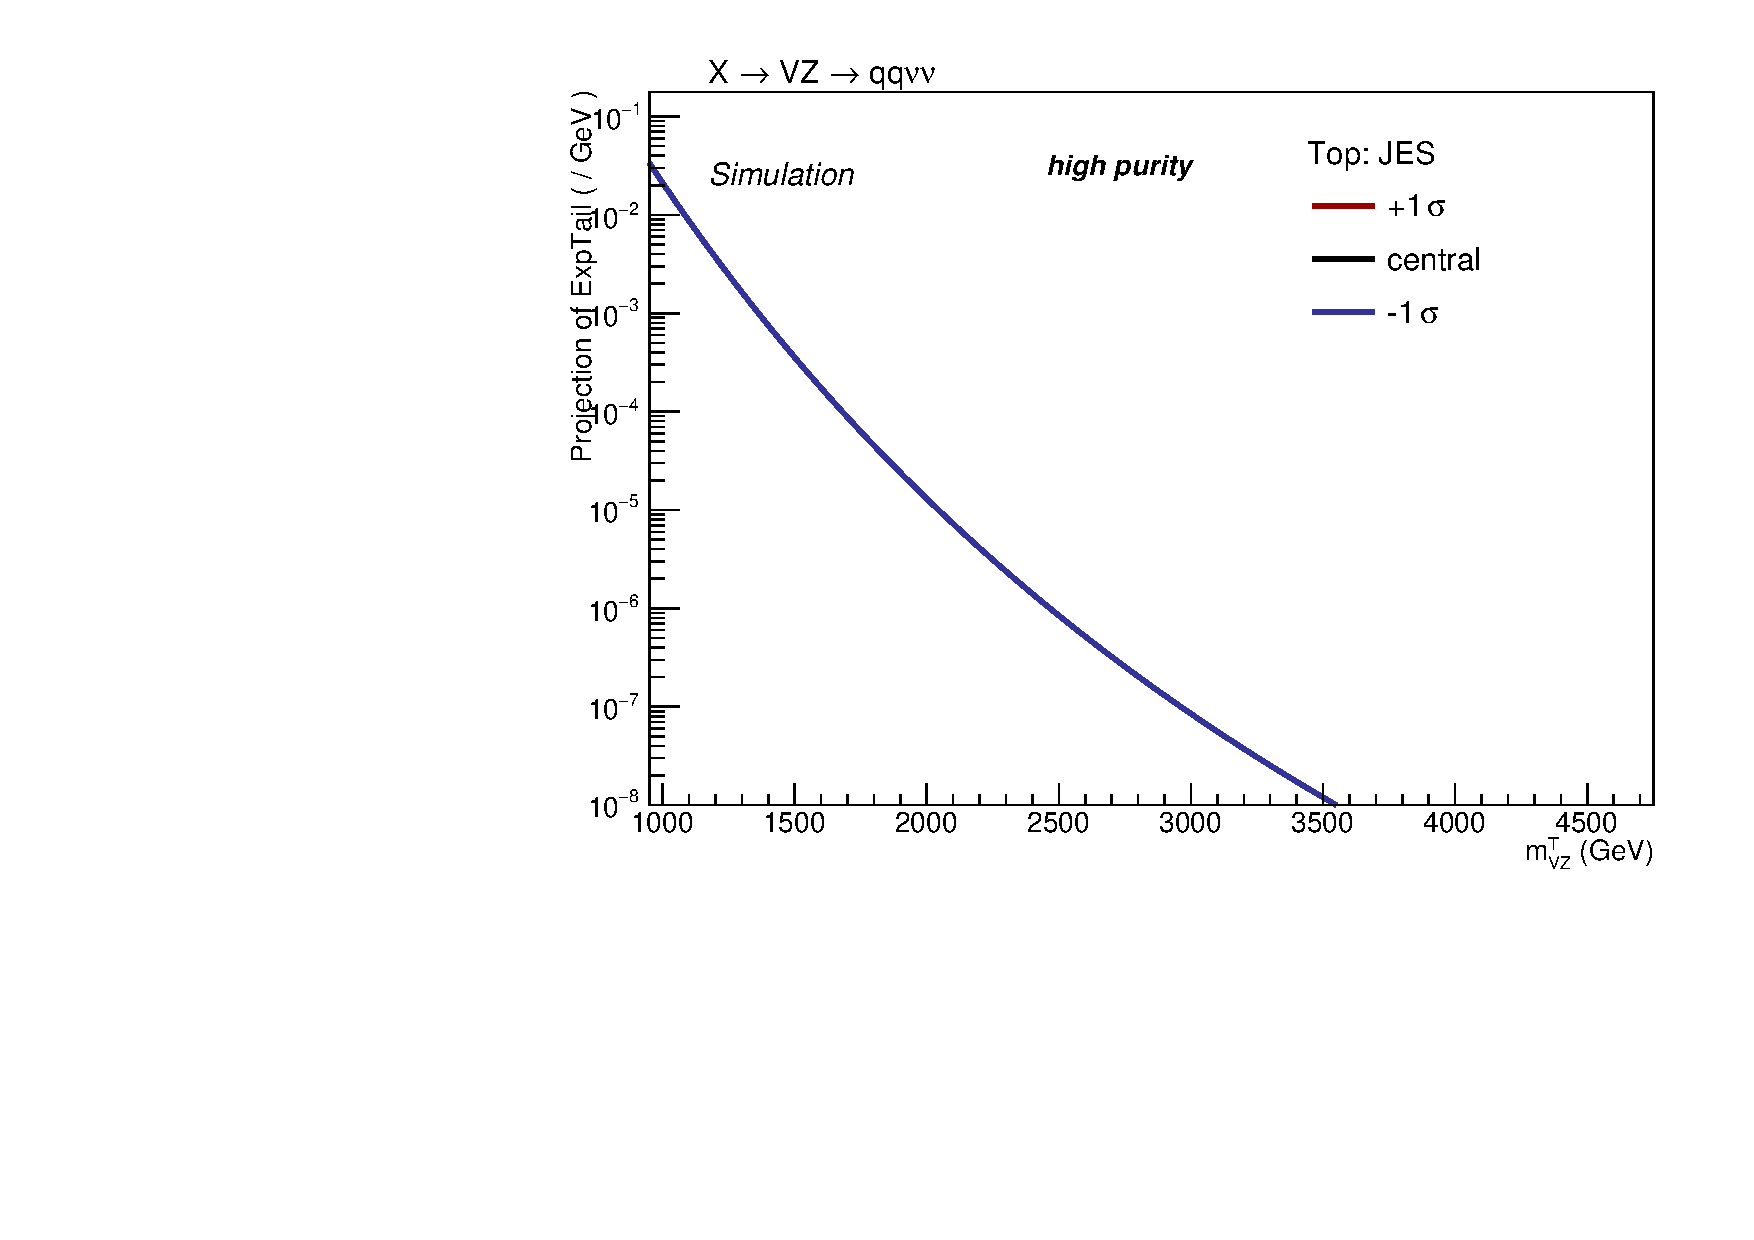
\includegraphics[width=.495\textwidth]{plots/Sys/SysTop_JES.pdf}
%     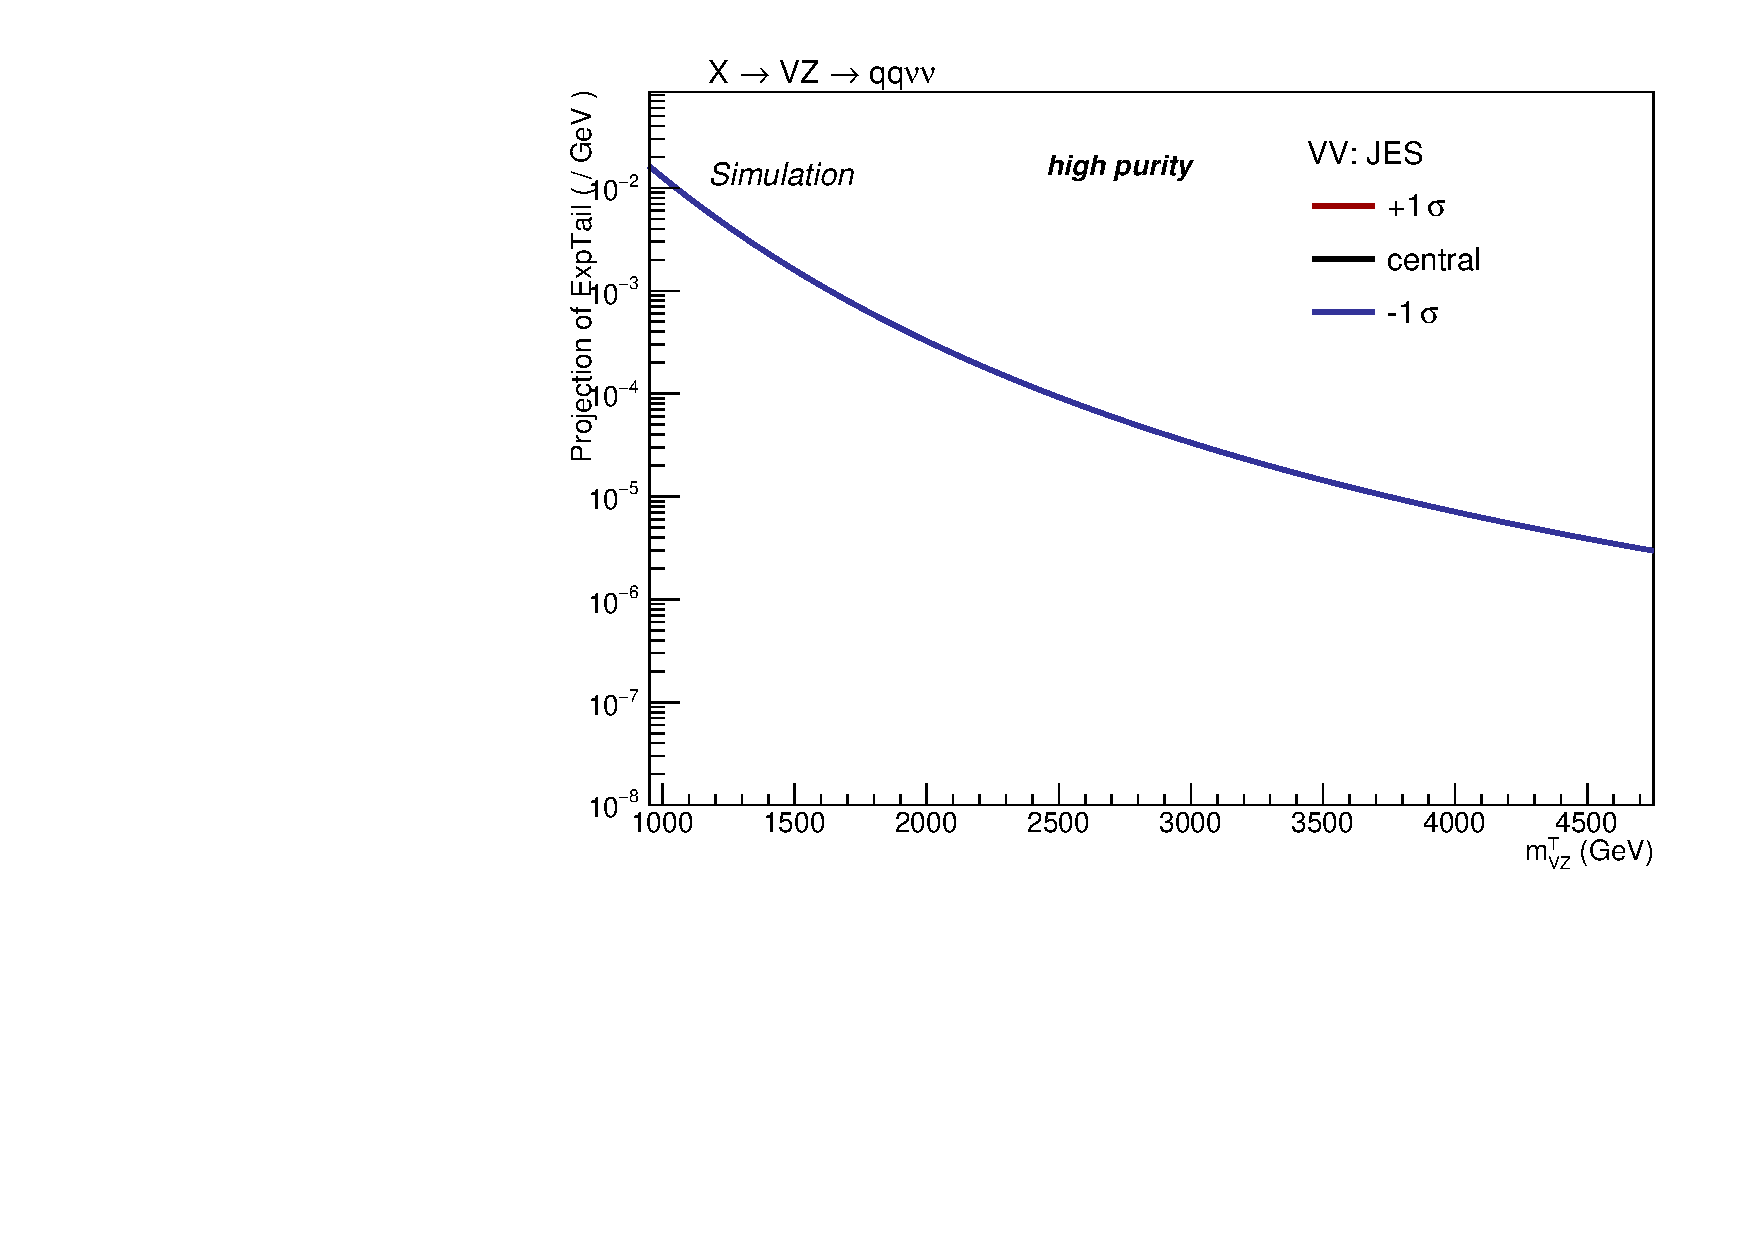
\includegraphics[width=.495\textwidth]{plots/Sys/SysVV_JES.pdf}
%   \end{center}
%   \caption{Shape variations due to JEC uncertainties obtained in the Top (left) and diboson (right) backgrounds.}
%   \label{fig:sysJES}
% \end{figure}

\subsubsection{Jet mass uncertainties}
\noindent The soft drop PUPPI corrected jet mass is affected by two different uncertainties sources.

\noindent Soft drop jet mass calibration is varied within $\pm \sqrt{ \left( \text{JES}_\text{unc.}^2 + \text{JMS}_\text{unc.}^2 \right) }$, where $\text{JES}_\text{unc.}$ is the uncertainty of the JES, described above, and $\text{JMS}_\text{unc.}=0.0094$ is a constant coefficent (~\ref{ssec:jetmass},\cite{bib:1748-0221-6-11-P11002},~\cite{CMS-DP-2016-020}). The impact is calculated on signal and secondary backgrounds, both in normalization and shape.

\noindent As regarding the smearing, the soft drop PUPPI corrected jet mass of the signal samples and sub-dominant backgrounds has been smeared up or down by a smearing coefficient (described in sec.~\ref{ssec:jetmass}), that is $ \text{JMR} = 1.00 \pm 0.20$.
\begin{table}[!htb]
  \centering
  \caption{Summary of jet mass energy corrections systematic uncertainties (JMS). The symbol $\Delta$ indicates the variation for each variable, due to the considered systematic uncertainty shift. \label{tab:jet_mass_energy_corr}}
  \begin{tabular}{l|cc}
	%& \multicolumn{2}{c}{ }\\
	\mtVZ & 1 TeV & 4 TeV \\
        \hline
	\hline
	$\Delta$ events & 1.0\% & 1.0\% \\
	$\Delta$ mean & 0.1\%& 0.1\% \\
	$\Delta$ RMS & $<$0.1\% & 0.4\% \\
	\hline
	secondary background & \VV & Top \\
        \hline
	$\Delta$ events & 0.1\% & 0.7\% \\
	$\Delta$ slope & $<$0.1\% & 0.2\% \\
  \end{tabular}

\end{table}


\begin{table}[!htb]
  \centering
  \caption{Summary of et mass resolution corrections systematic uncertainties (JMR). The symbol $\Delta$ indicates the variation for each variable, due to the considered systematic uncertainty shift. \label{tab:jet_mass_res_corr}}
  \begin{tabular}{l|cc}
	%& \multicolumn{2}{c}{ }\\
	\mtVZ & 1 TeV & 4 TeV \\
        \hline
	\hline
	$\Delta$ events & 5.2\% & 4.9\% \\
	$\Delta$ mean & 0.1\%& 0.1\% \\
	$\Delta$ RMS & 0.4\% & 0.3\% \\
	\hline
	secondary background & \VV & Top \\
        \hline
	$\Delta$ events & 2.0\% & 3.1\% \\
	$\Delta$ slope & 1.0\% & 4.0\% \\
  \end{tabular}

\end{table}

 \begin{figure}[!htb]
   \begin{center}
     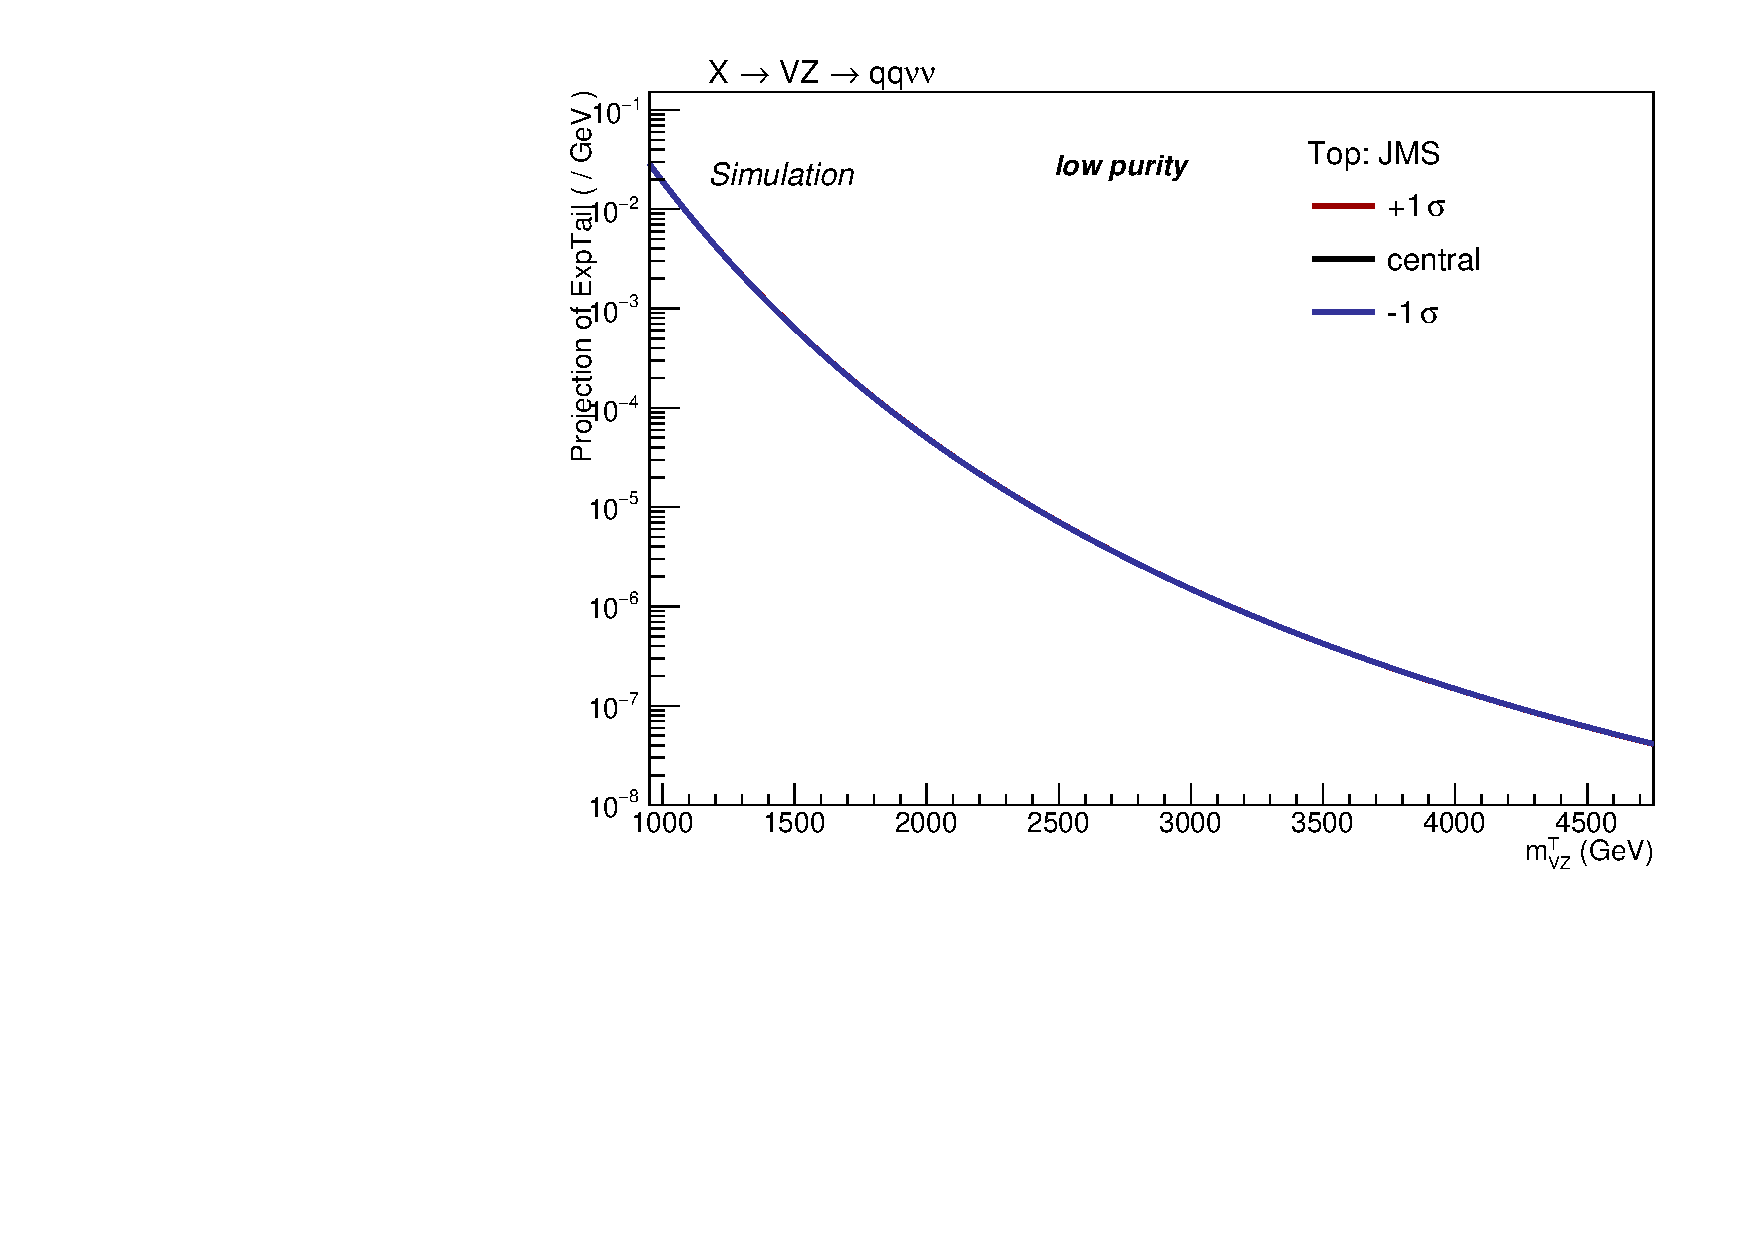
\includegraphics[width=.495\textwidth]{plotsAlpha_tesi/XVZnnlp/SysTop_JMS.pdf}
     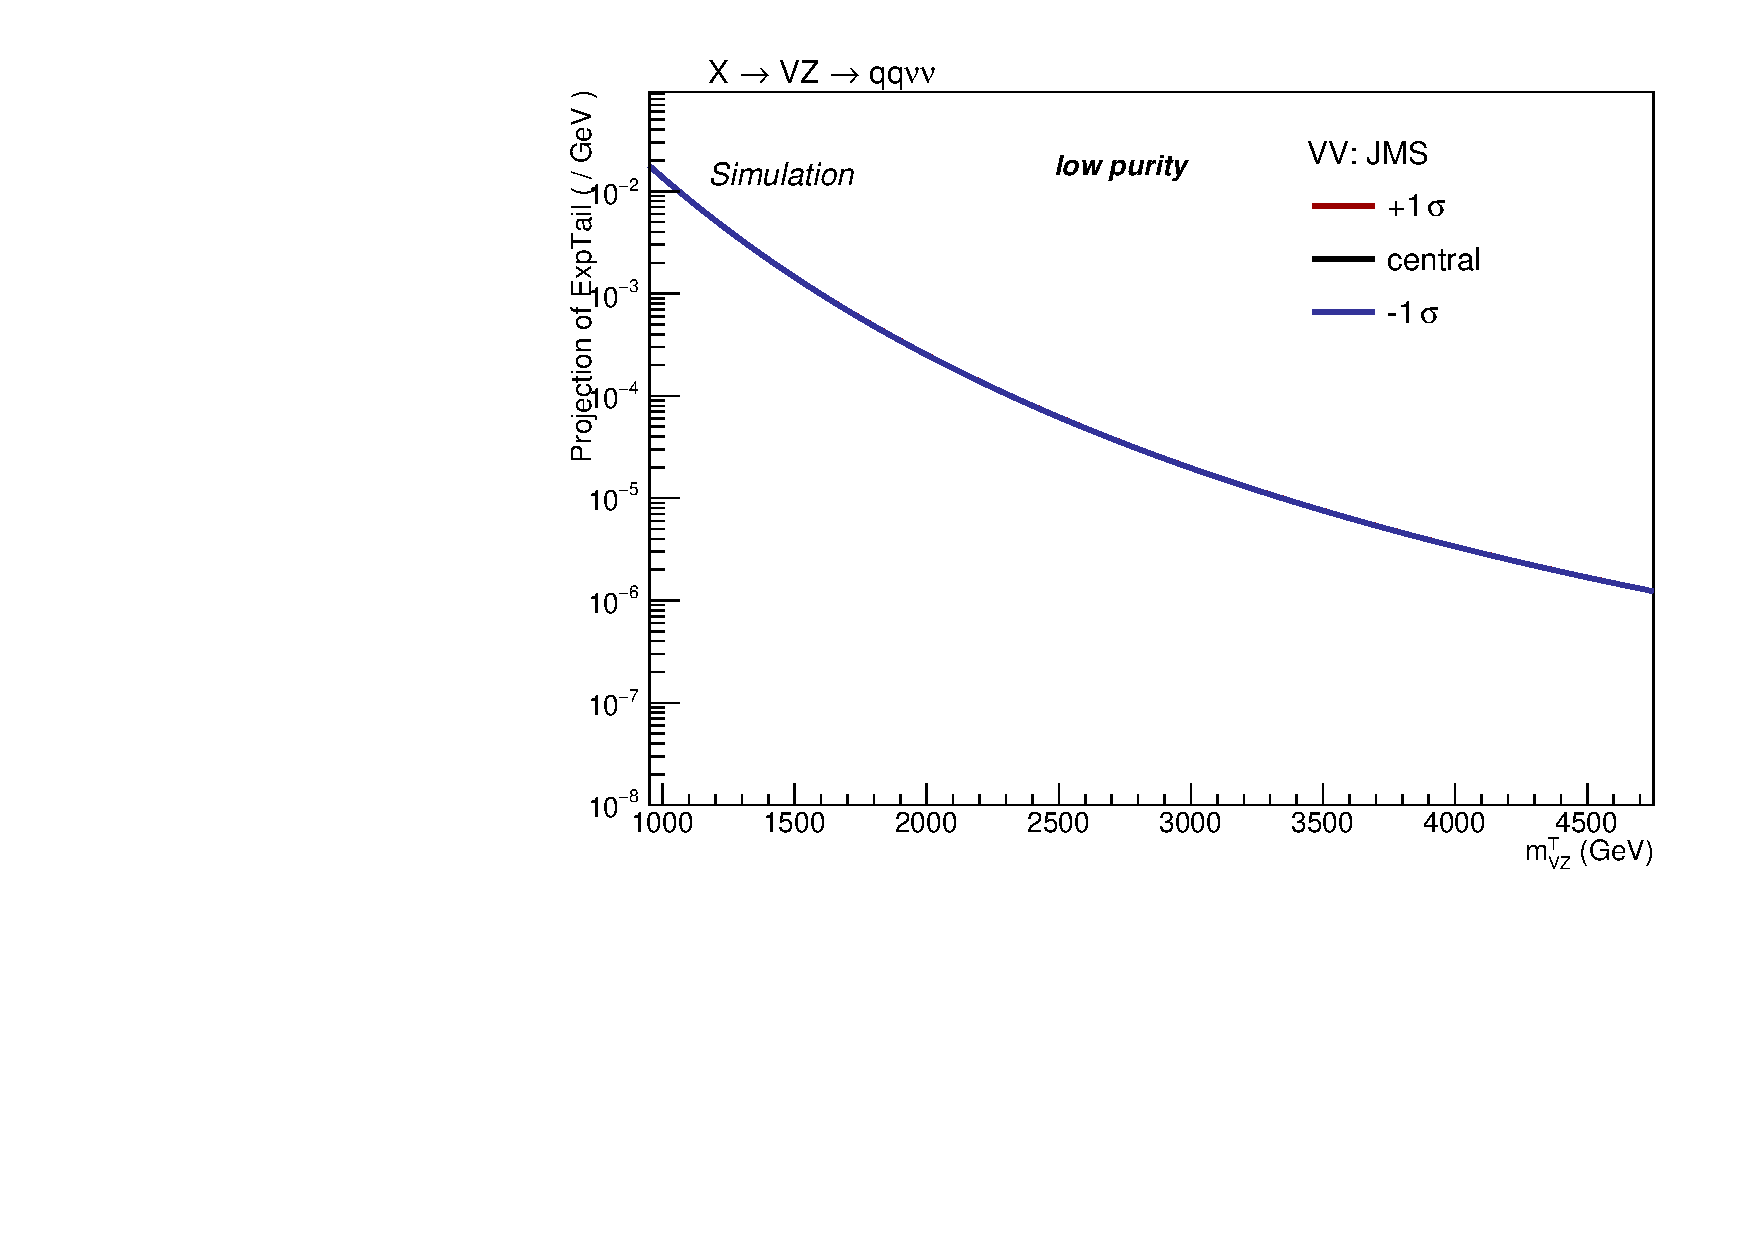
\includegraphics[width=.495\textwidth]{plotsAlpha_tesi/XVZnnlp/SysVV_JMS.pdf}
     \\
     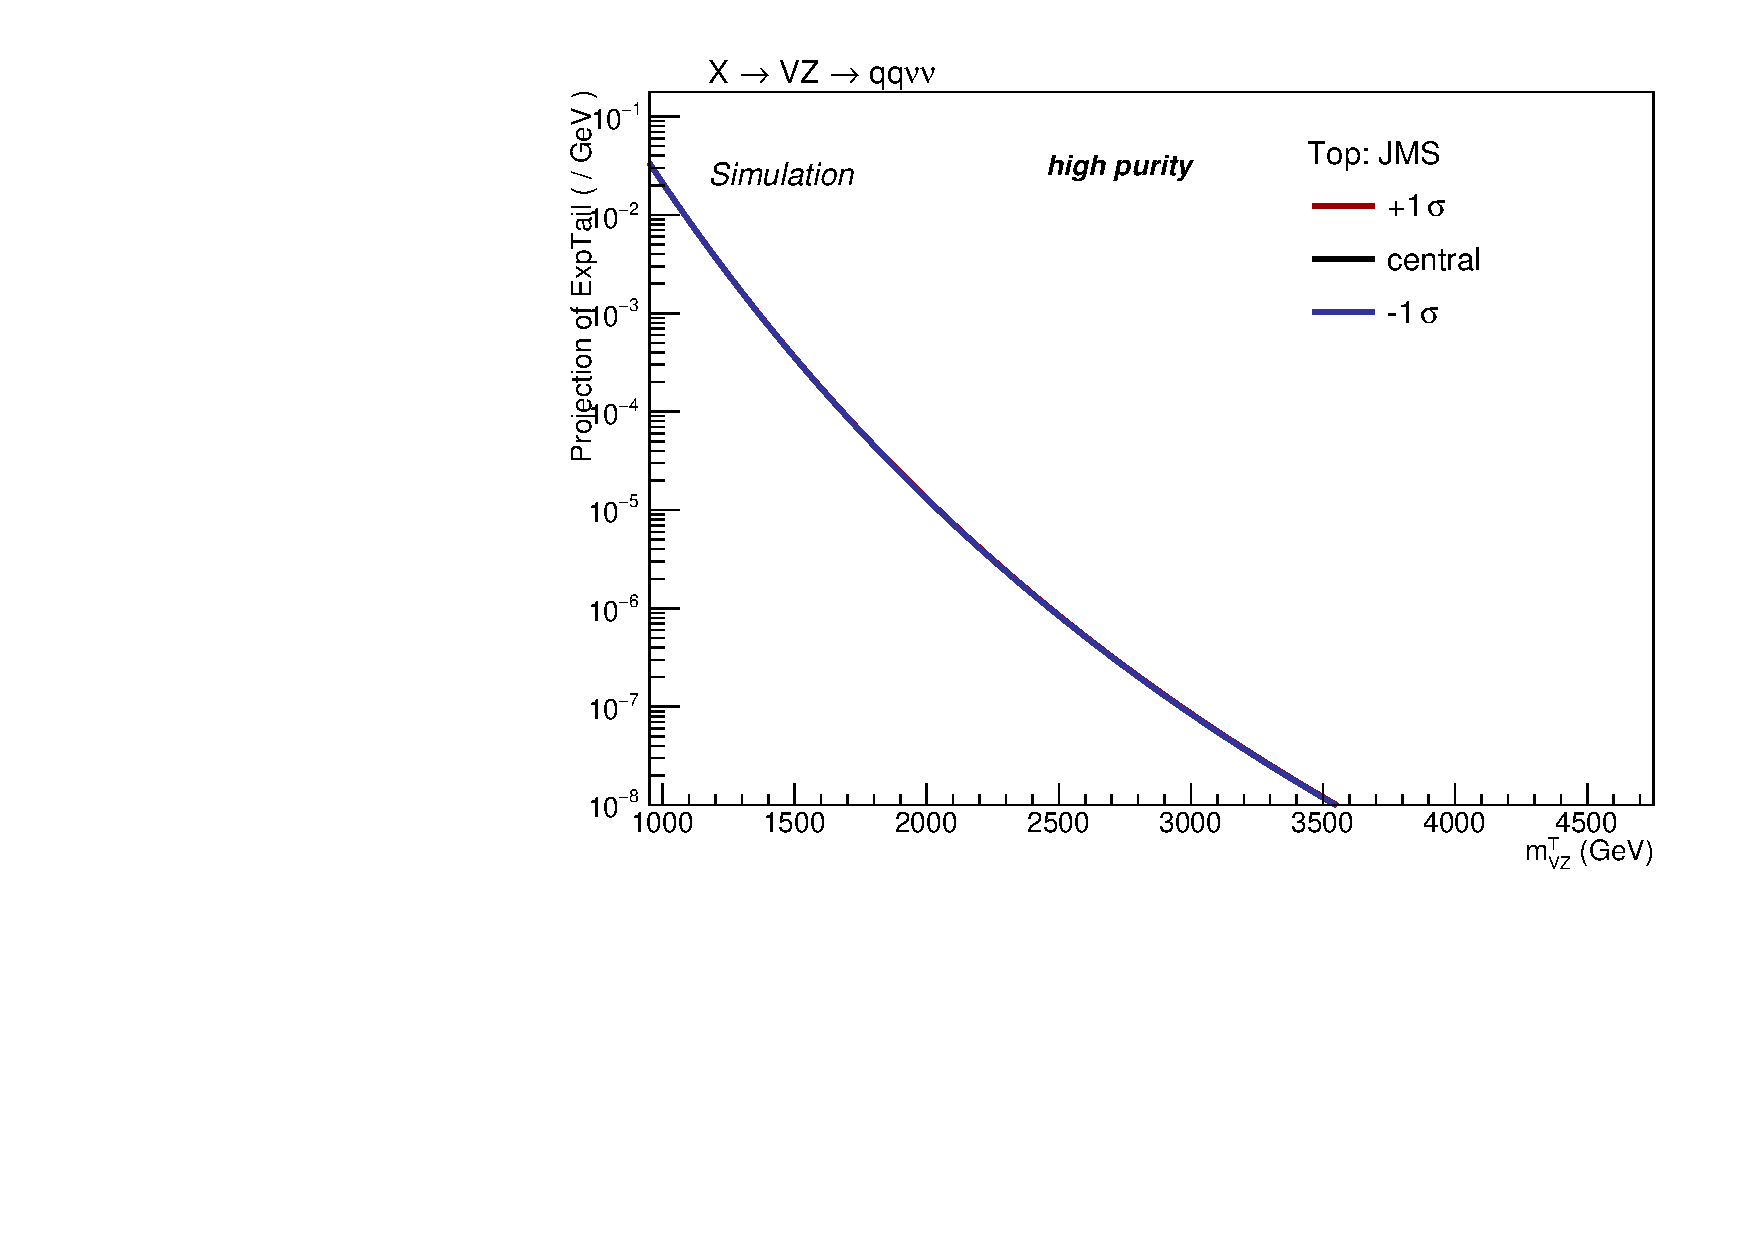
\includegraphics[width=.495\textwidth]{plotsAlpha_tesi/XVZnnhp/SysTop_JMS.pdf}
     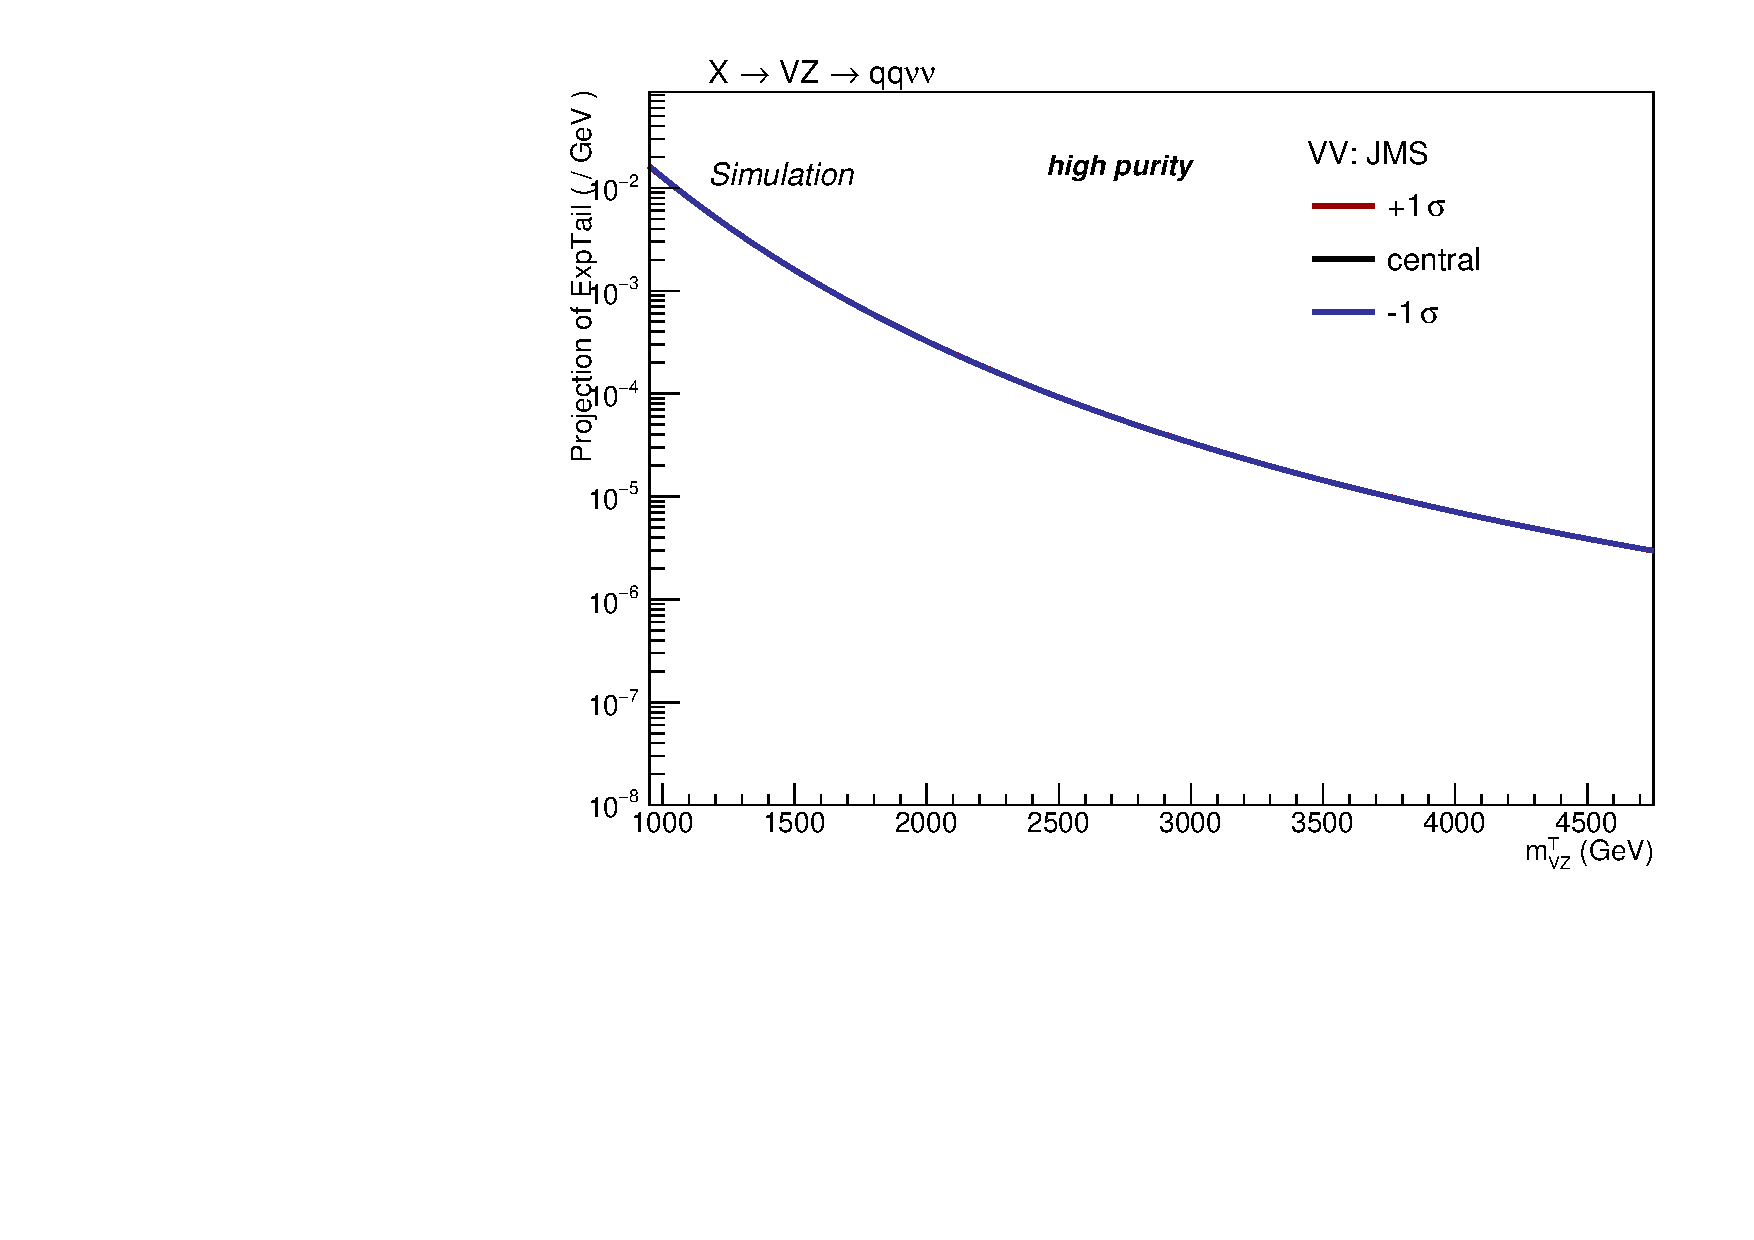
\includegraphics[width=.495\textwidth]{plotsAlpha_tesi/XVZnnhp/SysVV_JMS.pdf}

   \end{center}
   \caption{Shape variations due to jet mass calibration corrections obtained in the Top (left) and diboson (right) backgrounds, in the low-purity (top) and high-purity (bottom) category.}
   \label{fig:sysJMS}
 \end{figure}

 \begin{figure}[!htb]
   \begin{center}
     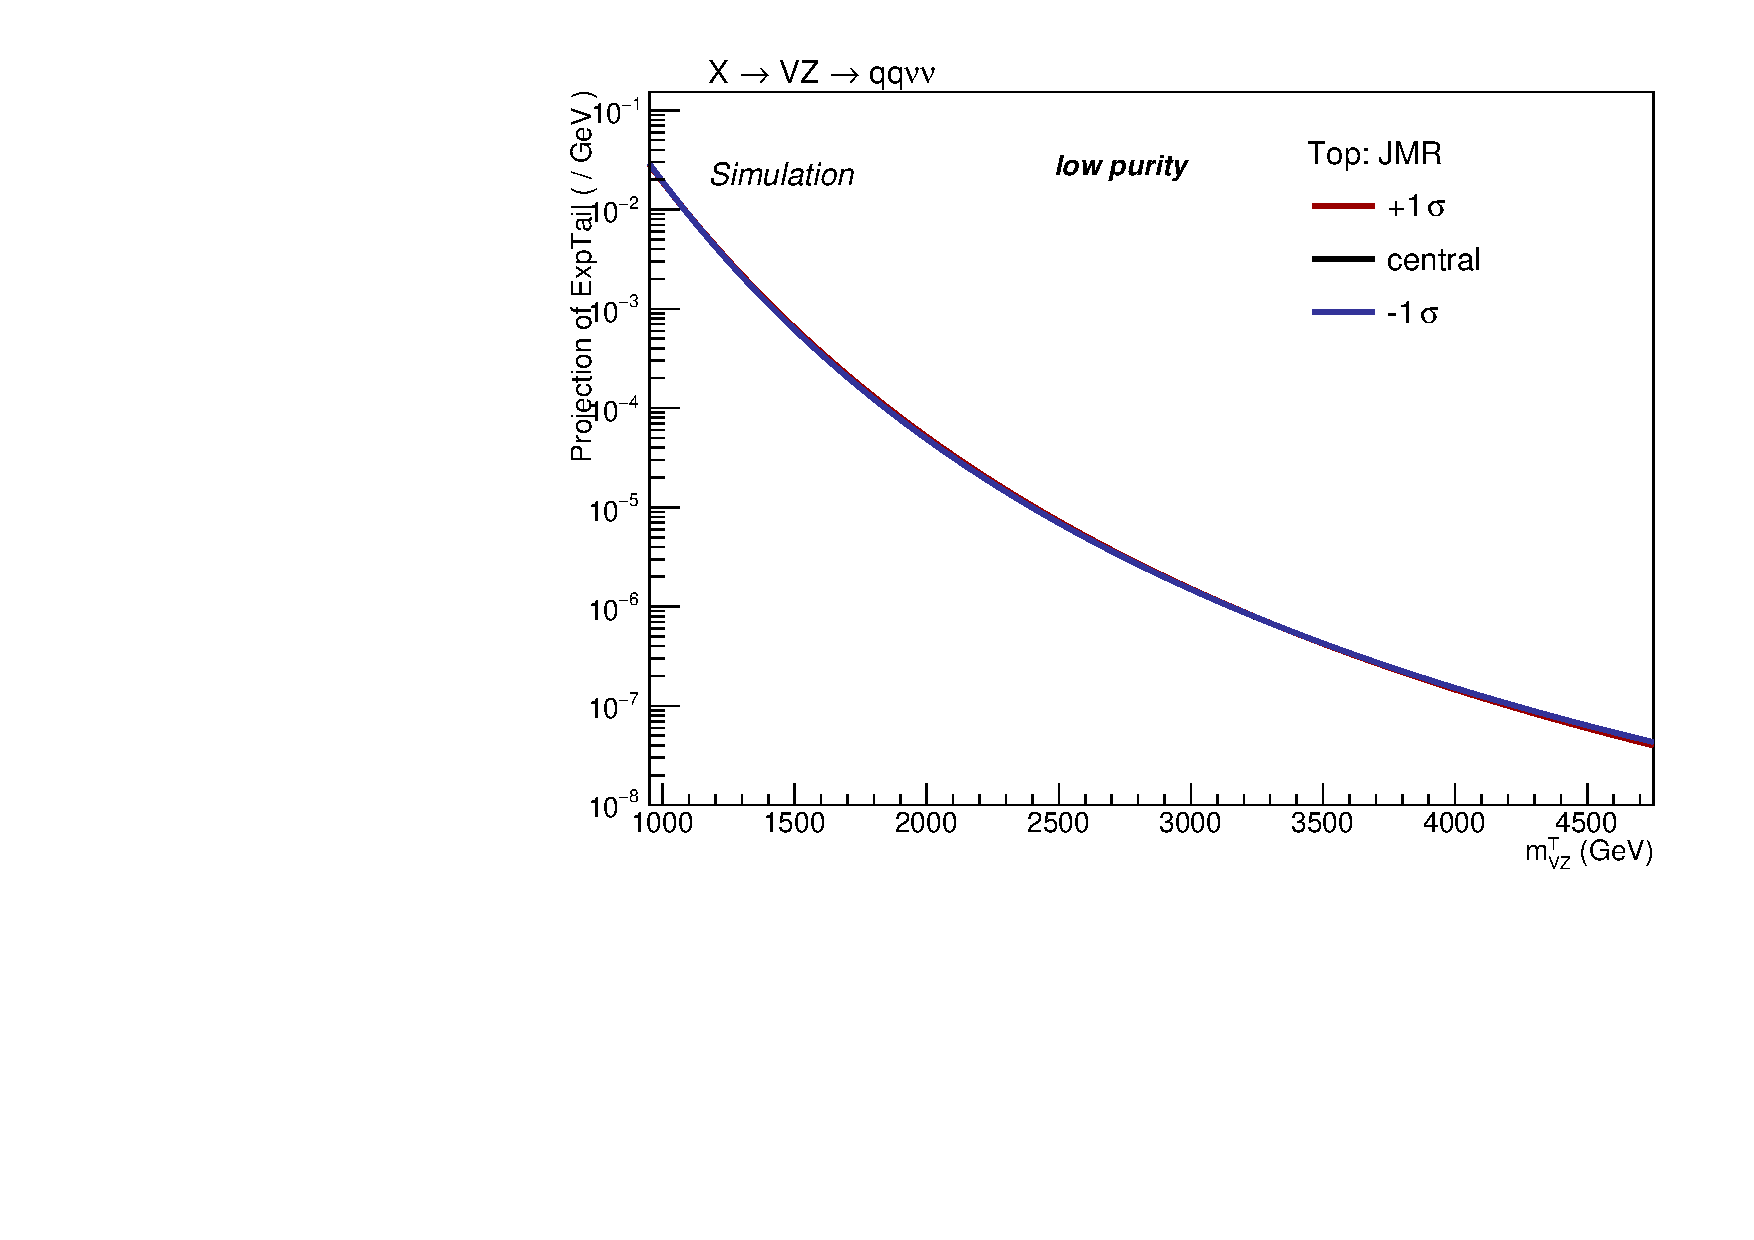
\includegraphics[width=.495\textwidth]{plotsAlpha_tesi/XVZnnlp/SysTop_JMR.pdf}
     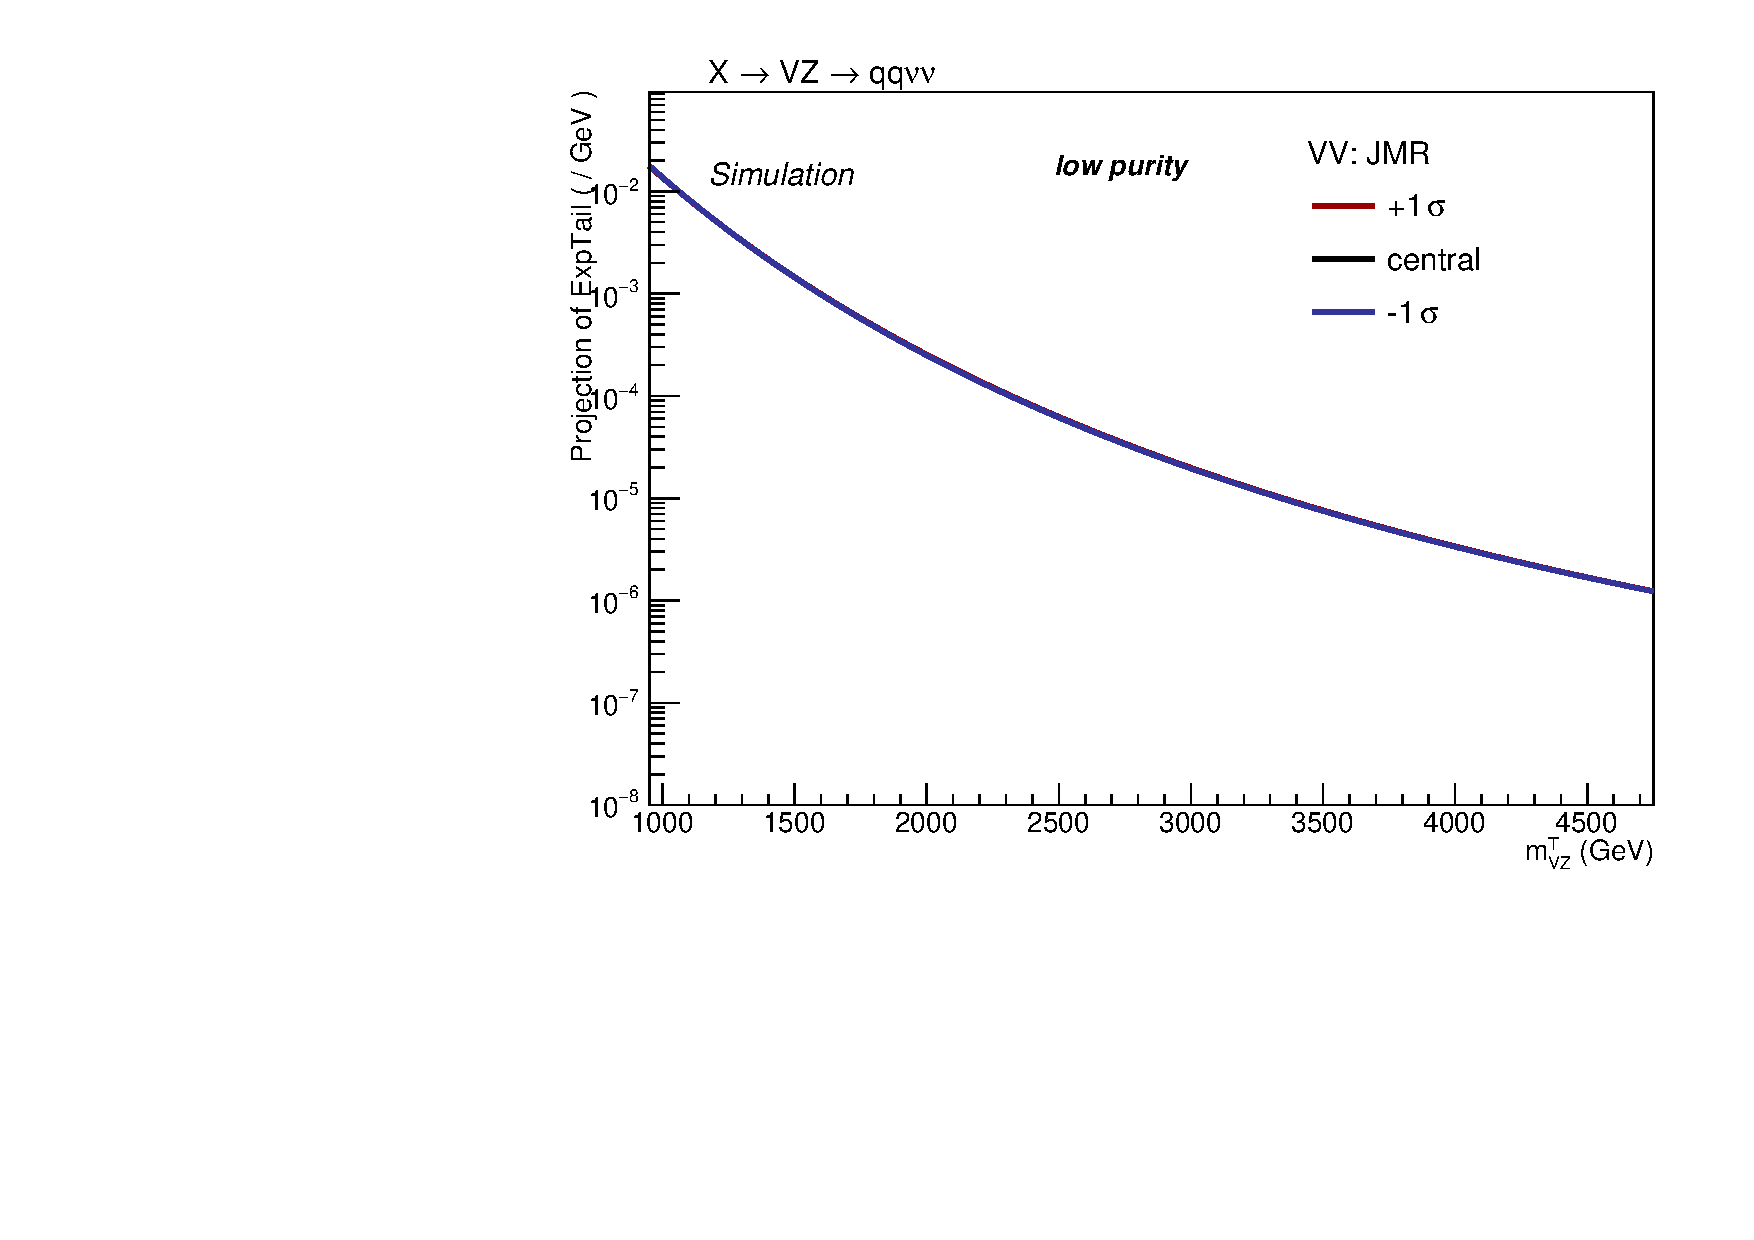
\includegraphics[width=.495\textwidth]{plotsAlpha_tesi/XVZnnlp/SysVV_JMR.pdf}
     \\
     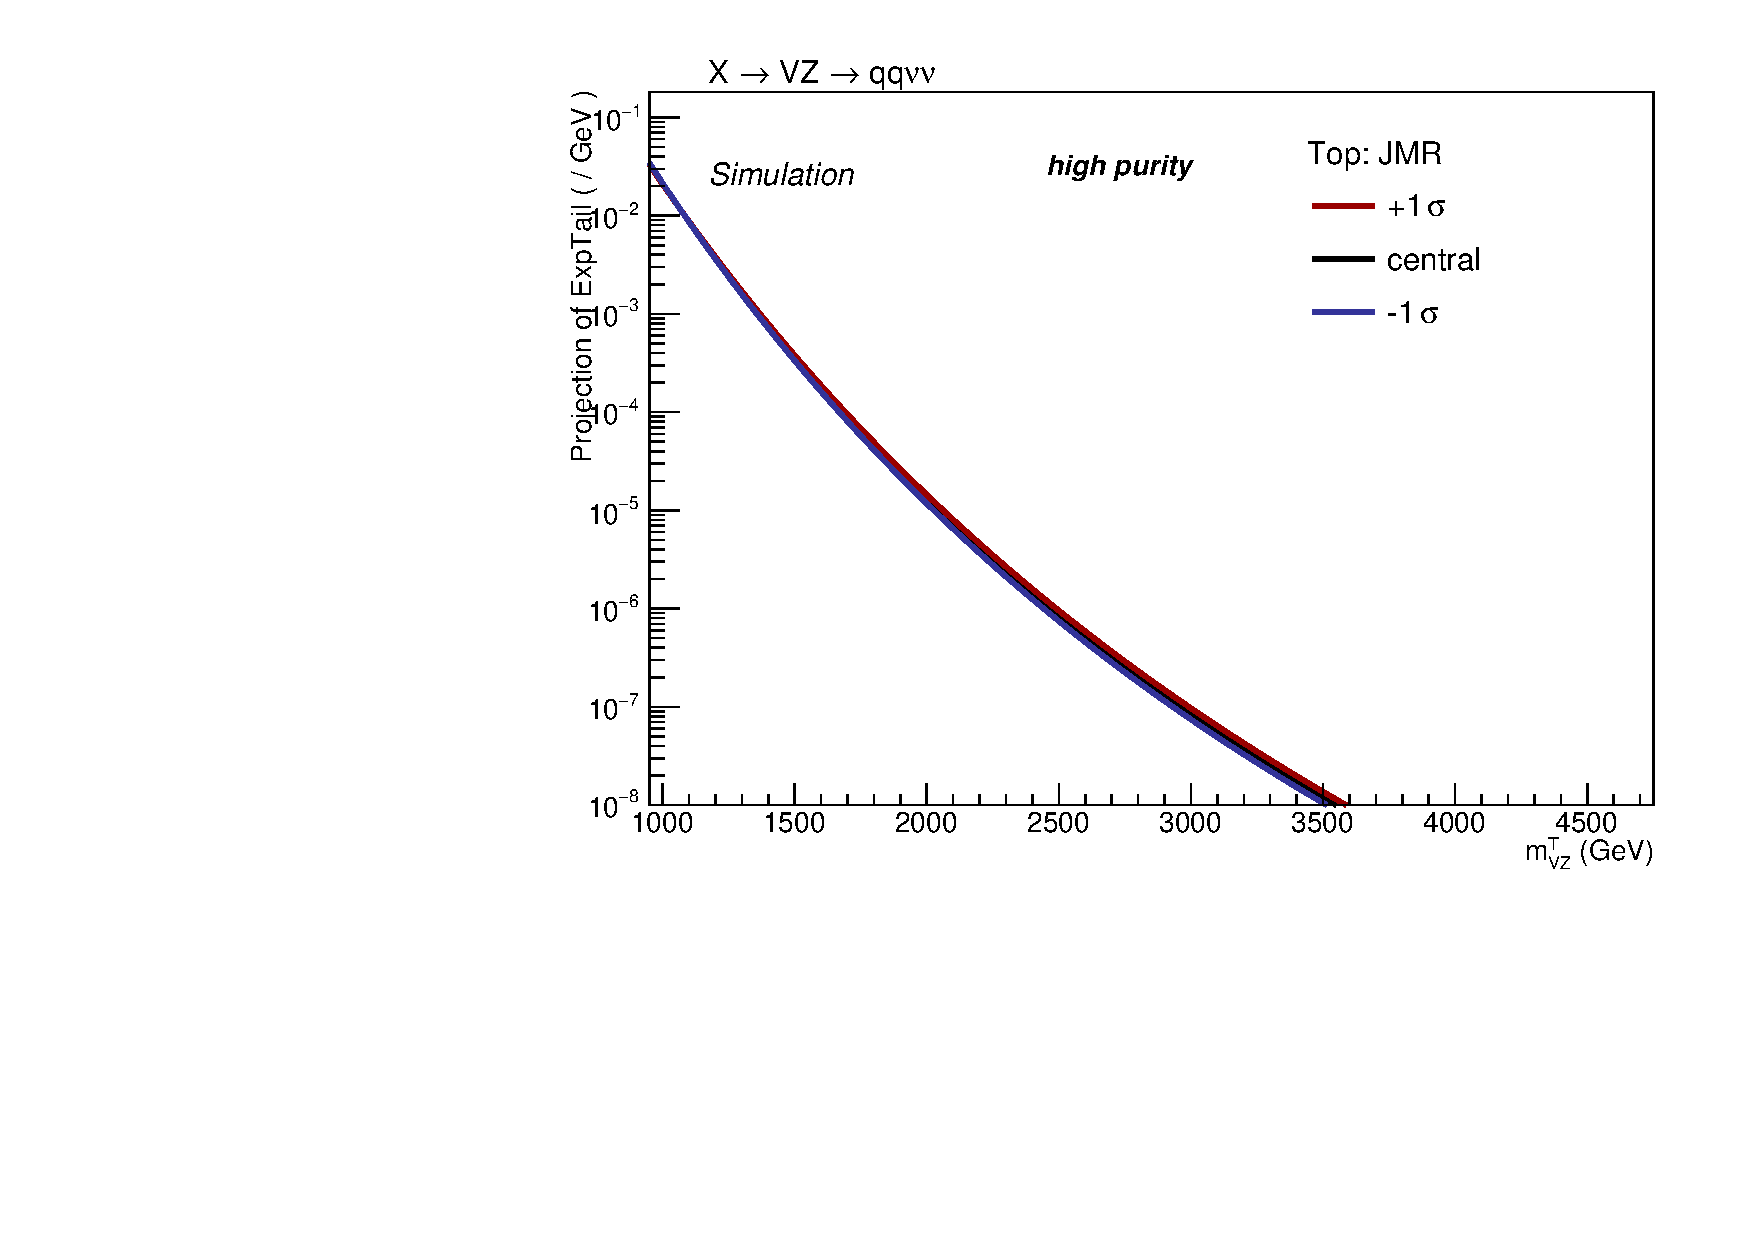
\includegraphics[width=.495\textwidth]{plotsAlpha_tesi/XVZnnhp/SysTop_JMR.pdf}
     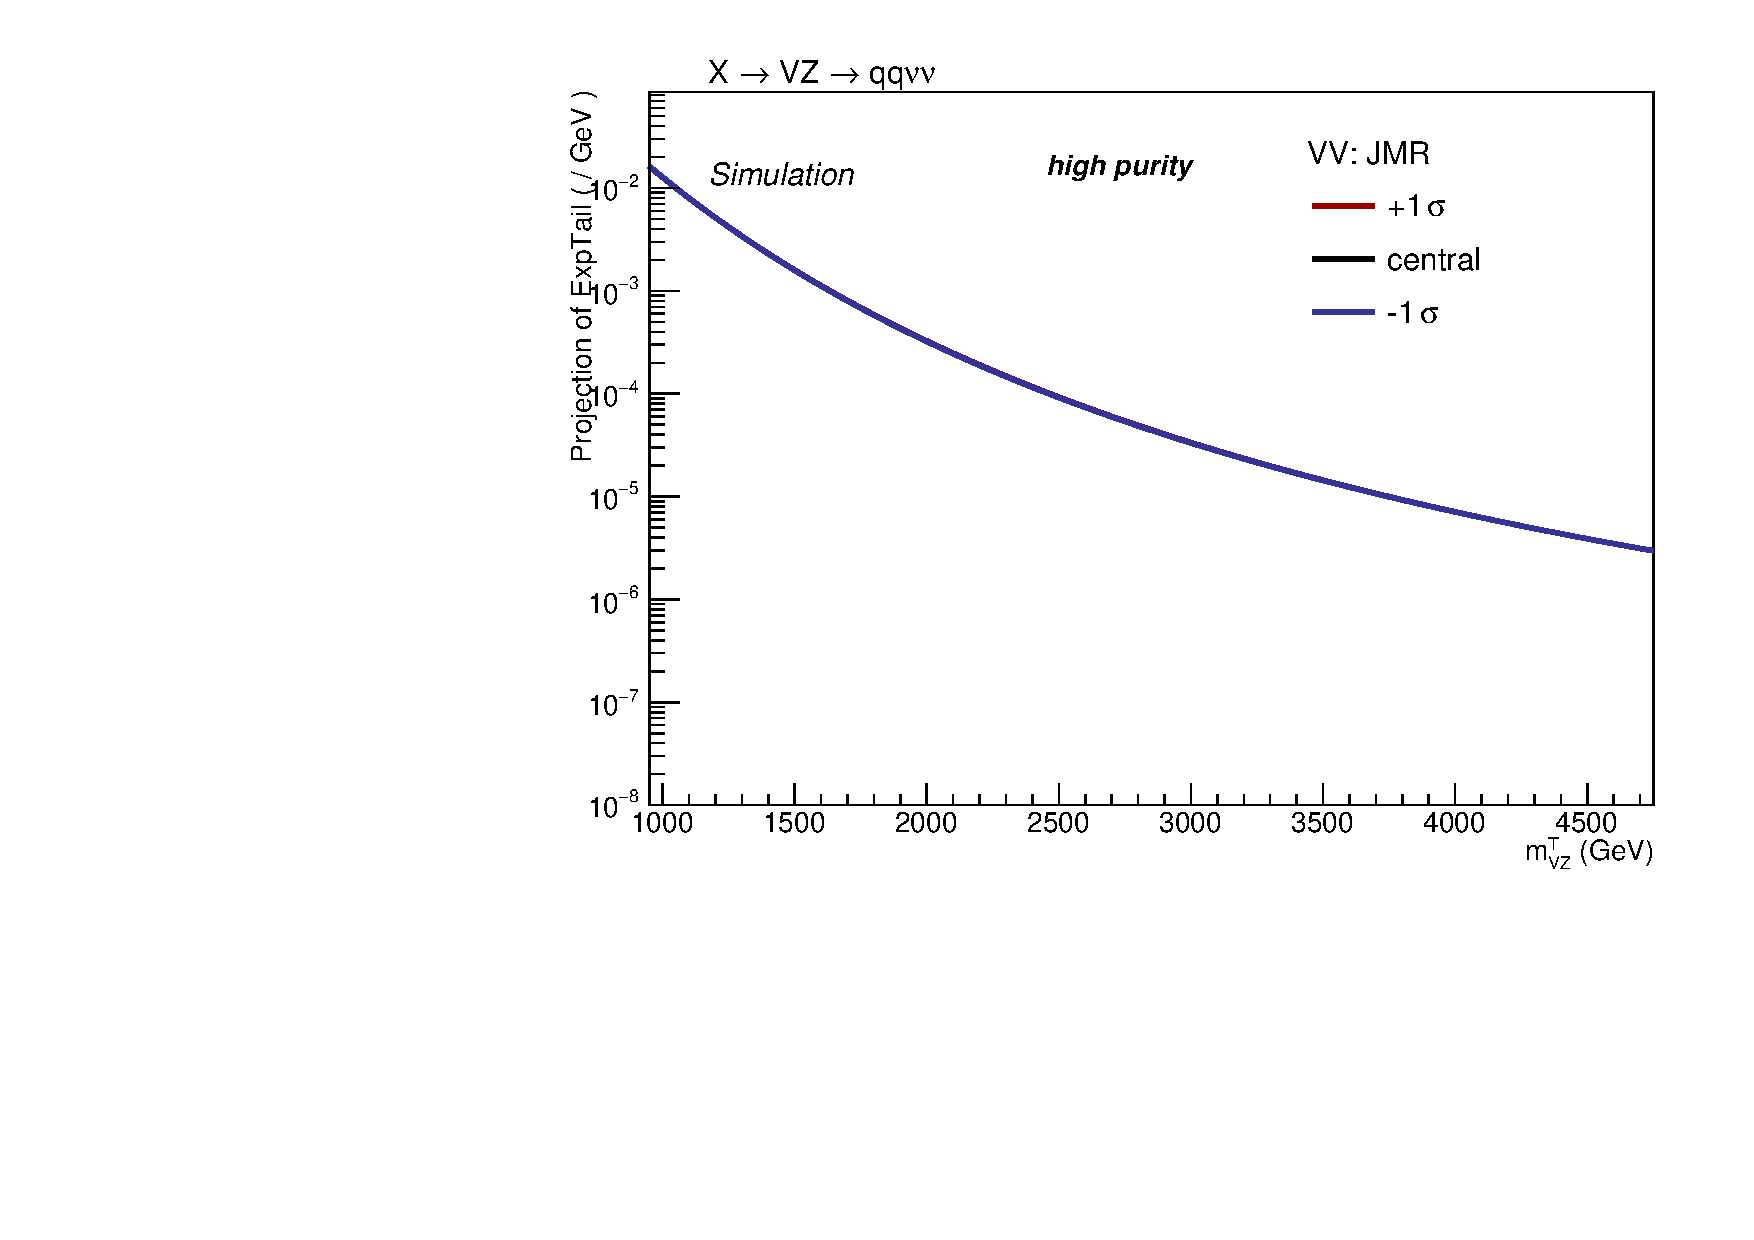
\includegraphics[width=.495\textwidth]{plotsAlpha_tesi/XVZnnhp/SysVV_JMR.pdf}

   \end{center}
   \caption{Shape variations due to jet mass resolution obtained in the Top (left) and diboson (right) backgrounds, in the low-purity (top) and high-purity (bottom) category.}
   \label{fig:sysJMR}
 \end{figure}

\noindent Results are presented in detail in tab.~\ref{tab:jet_mass_energy_corr}-\ref{tab:jet_mass_res_corr}, for JMS and JMR uncertainties. Shape uncertainties on signal are evaluated as the variation in the mean and variance of the transverse mass distribution. Shape uncertainties on top and diboson backgrounds are quoted as the relative variation in the slope of the exponential falling distribution of \mtVZ, and their effects are shown in fig. \ref{fig:sysJMS}-\ref{fig:sysJMR}.


\subsubsection{\V-tagging uncertainties}
\label{sec:wtagunc}

Data-Monte Carlo \V-tagging scale factors are applied to the signal and secondary background yields (sec.~\ref{ssec:jetsub_corr}), and their uncertainty is taken as systematic uncertainty. The contribution of the uncertainty is 11\% for the high-purity and 23\% for low-purity category, applied on signal and secondary backgrounds. While combining the categories, \V-tagging uncertainties are considered as anti-correlated.

\noindent The \V-tagging scale factors are measured in \ttbar samples, hence at \pt values generally not larger than 200--300 \GeV. An uncertainty due to the \V-tagging extrapolation at higher momenta is considered by using an alternative showering scheme (HERWIG~\cite{bib:HERWIG}). It is parametrized as a function of the jet \pt: $X \times \log(\pt/200 \GeV)$, where $X=0.085$ for the high-purity category and $X=0.039$ for low-purity category. It amounts to 9-20\%, depending on the mass of the signal sample considered, to 2-3\% for \VV and Top backgrounds in high-low purity category. While combining the categories, \V-tagging extrapolation uncertainties are considered as correlated.


\subsubsection{b-tagging uncertainties}
\label{sec:btagunc}
The assigned b-tagging uncertainty, related to the b-tag veto applied to AK4 jets that lie outside the \V jet cone, with the aim of suppressing the top quark induced background, is the relative difference in shape and normalization, calculated in signal and secondary background events, obtained by shifting up or down the event weight through the envelope of the data-MC b-tagging scale factors uncertainties~\cite{bib:btagsf}.

\noindent The impact of this systematic uncertainty on signal normalization ranges from 0.7\% at 1 \TeV, up to 1.0\% at 4 \TeV. The impact on \VV background normalization is 0.3\%, whilst on Top it is 2.2\%. Effects on signal and background shapes are negligible.

\subsubsection{Missing Energy uncertainties}
\label{metuncsec}
As described in sec.~\ref{ssec:met_description}, the \MET evaluation depends on all the reconstructed particles in the event, and on their uncertainties. Missing energy uncertainties are calculated by factorizing \met in components: electrons, photons, muons, taus, jets and unclustered energy. Dedicated uncertainties are derived by propagating the original object scales and resolutions to the \MET itself.

\noindent In this analysis, a leptonic veto is applied, hence the \MET uncertainties are due to jets and unclustered energy. The effect of JES is evaluated on \MET in a correlated way with jets, by scaling up or down the central value of JES by one sigma, both on \MET and on jets \pt. The result is a neglibile uncertainty on signal normalization, 0.2\% and less than 0.1\% uncertainty on top and diboson normalizations, negligible impact on signal, top and diboson shapes.

\noindent The same procedure applies for the uncertainties related to jet JER, that are varied up and down by one sigma in both jets and \met at the same time. The result is a negligible uncertainty on signal and diboson normalizations, 0.3\% uncertainty on top normalization, and negligible effects on signal and background shapes.

\noindent The last contribution in \MET uncertainty is related to unclustered energy, whose impact is evaluated scaling up or down the central value by its own resolution, depending on the particle type. The uncertainty is negligible on signal and background normalizations and shape.

\subsubsection{Pile-up uncertainty}
An additional source of systematic uncertainty is the limited knowledge of the total proton-proton inelastic cross-section at $13$ \TeV, used to get the expected number of vertices distribution for the pile-up reweighting procedure. A $4.6\%$ uncertainty is assumed for the default value of $69.2$ mb, and the vertices distributions are varied accordingly (fig.~\ref{fig:PU_updown}). Changing the pile-up weight varies also the MC normalizations in the signal region, and the relative difference is estimated to be 0.2\% for the diboson background, 0.3\% for top processes, and 0.4-0.7\% for signal samples. Pile-up impacts on signal shapes are negligible, and it affects by 0.8\% and 0.4\% the diboson and top shapes (fig.~\ref{fig:syspileup}). %No shape uncertainties are considered for PU. %$3\%$ for the diboson and top samples, and a flat $0.5\%$ for signal samples. No shape uncertainties are considered for PU.

\begin{figure}[!htb]
  \begin{center}
    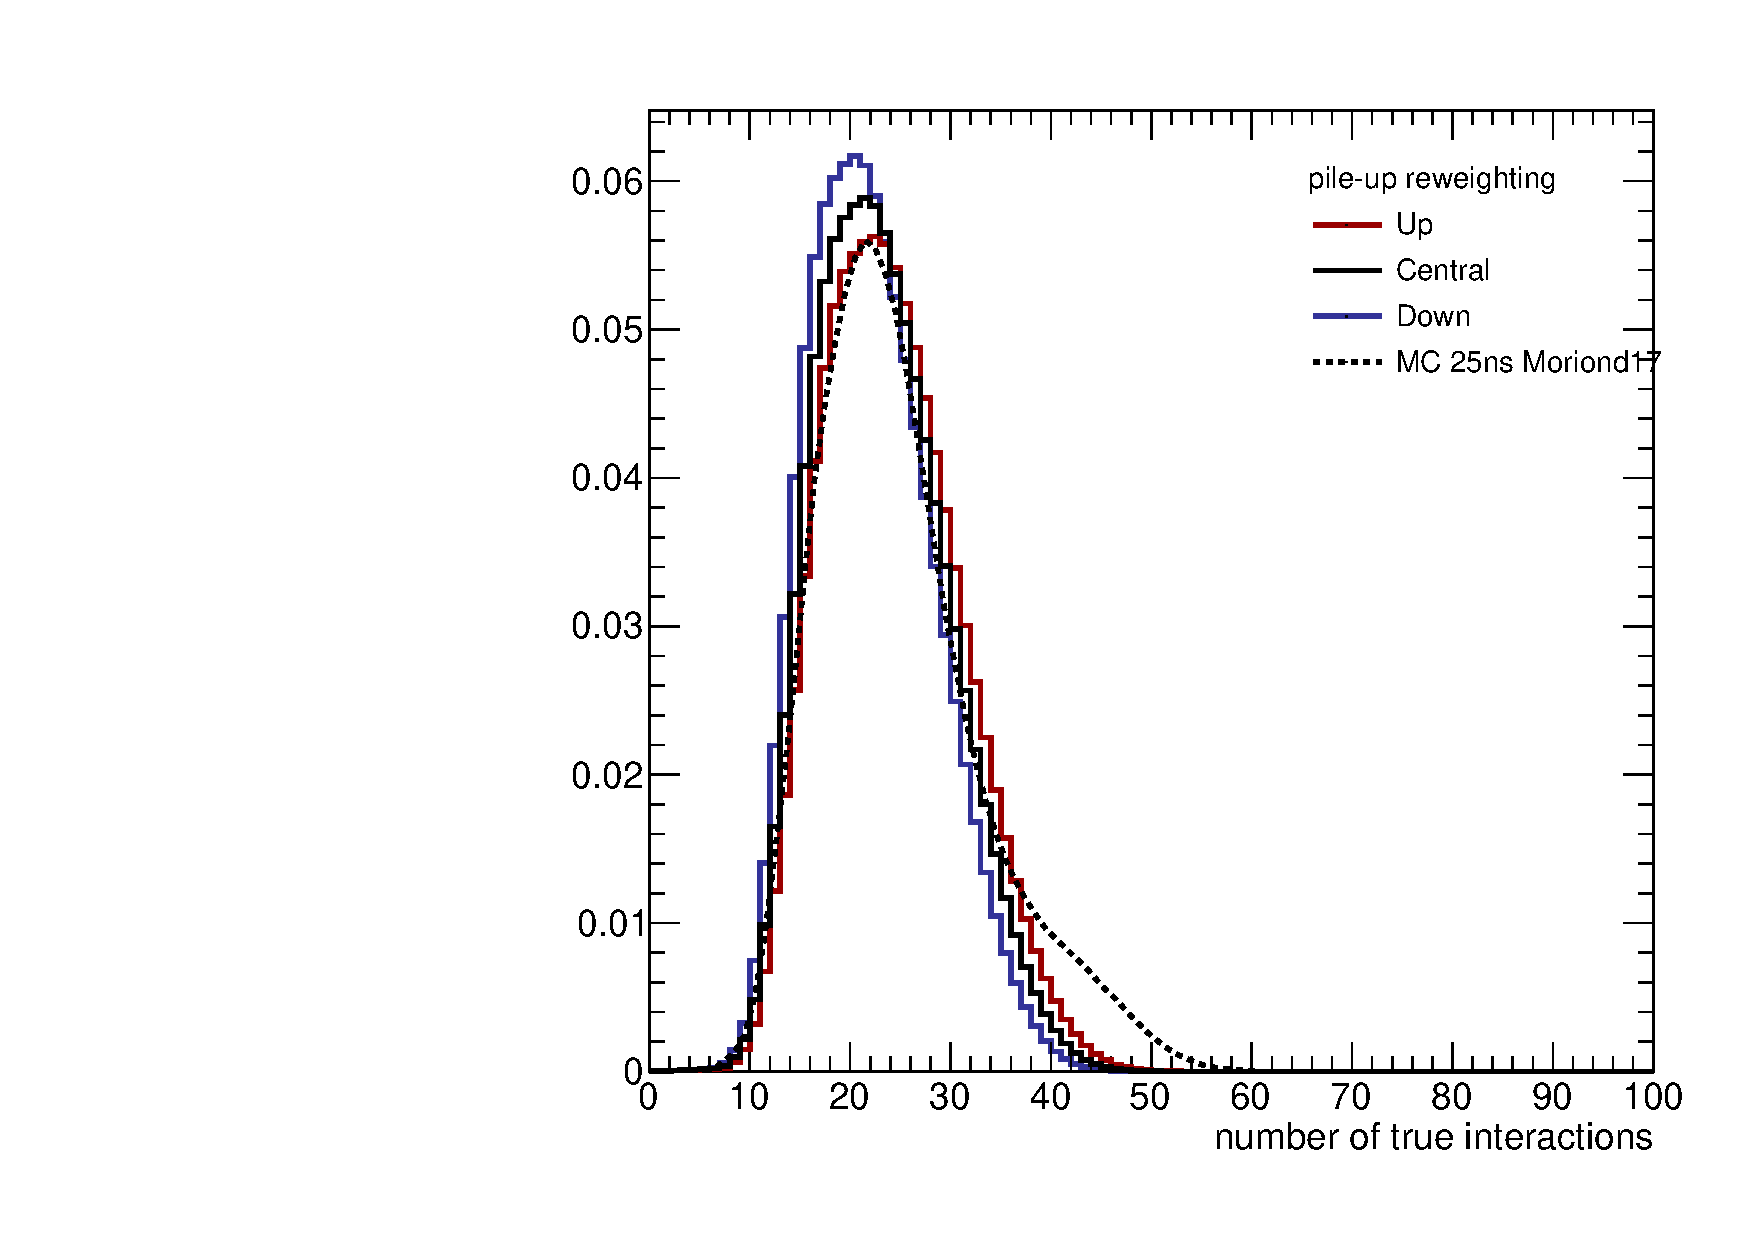
\includegraphics[width=.495\textwidth]{figures/PU_Moriond17.pdf}
  \end{center}
  \caption{Pile-up scenario in 2016 data (black curve), and scenarios obtained by shifting up (red curve) or down (blue curve) the central value of the total inelastic cross-section ($69.2$ mb), compared to pile-up distribution simulated in Monte Carlo samples (dotted curve).}
  \label{fig:PU_updown}
\end{figure}

 \begin{figure}[!htb]
   \begin{center}
     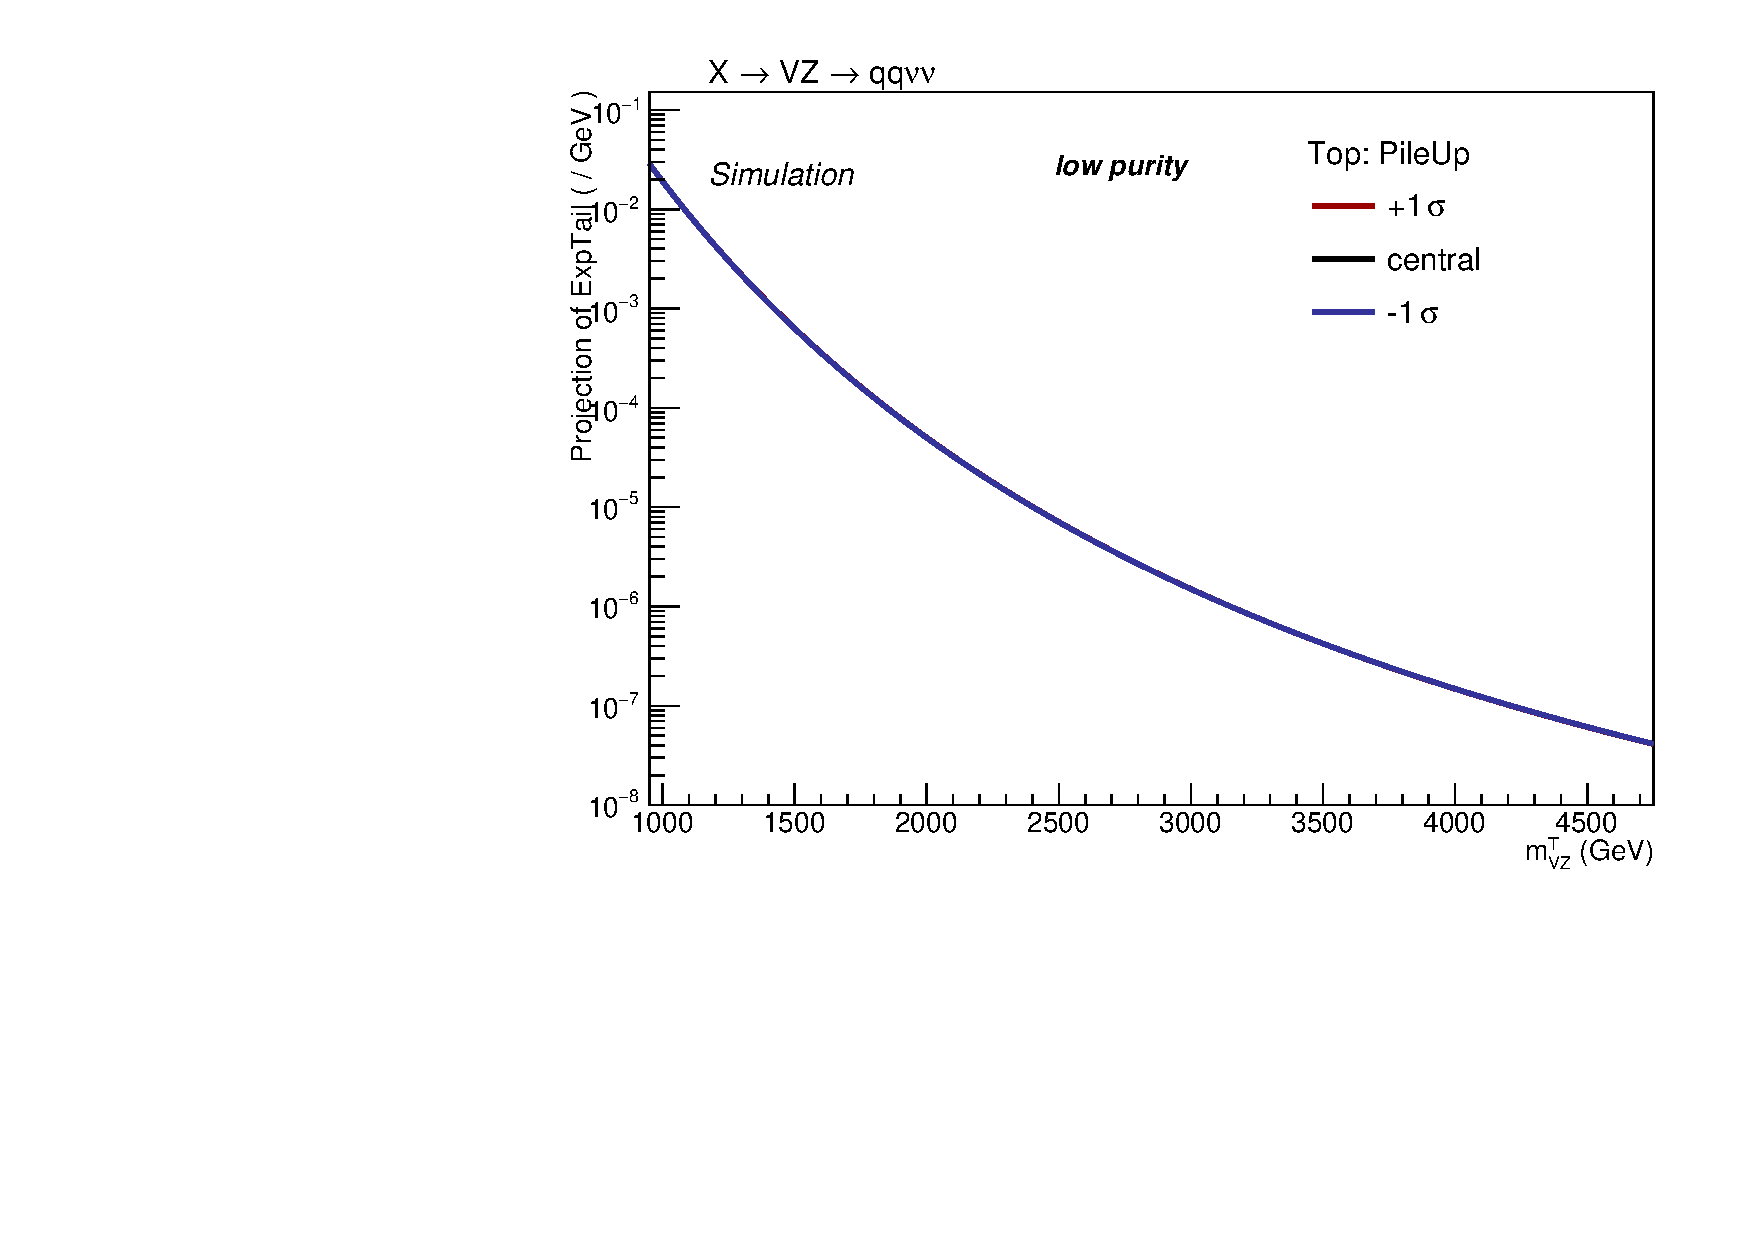
\includegraphics[width=.495\textwidth]{plotsAlpha_tesi/XVZnnlp/SysTop_PileUp.pdf}
     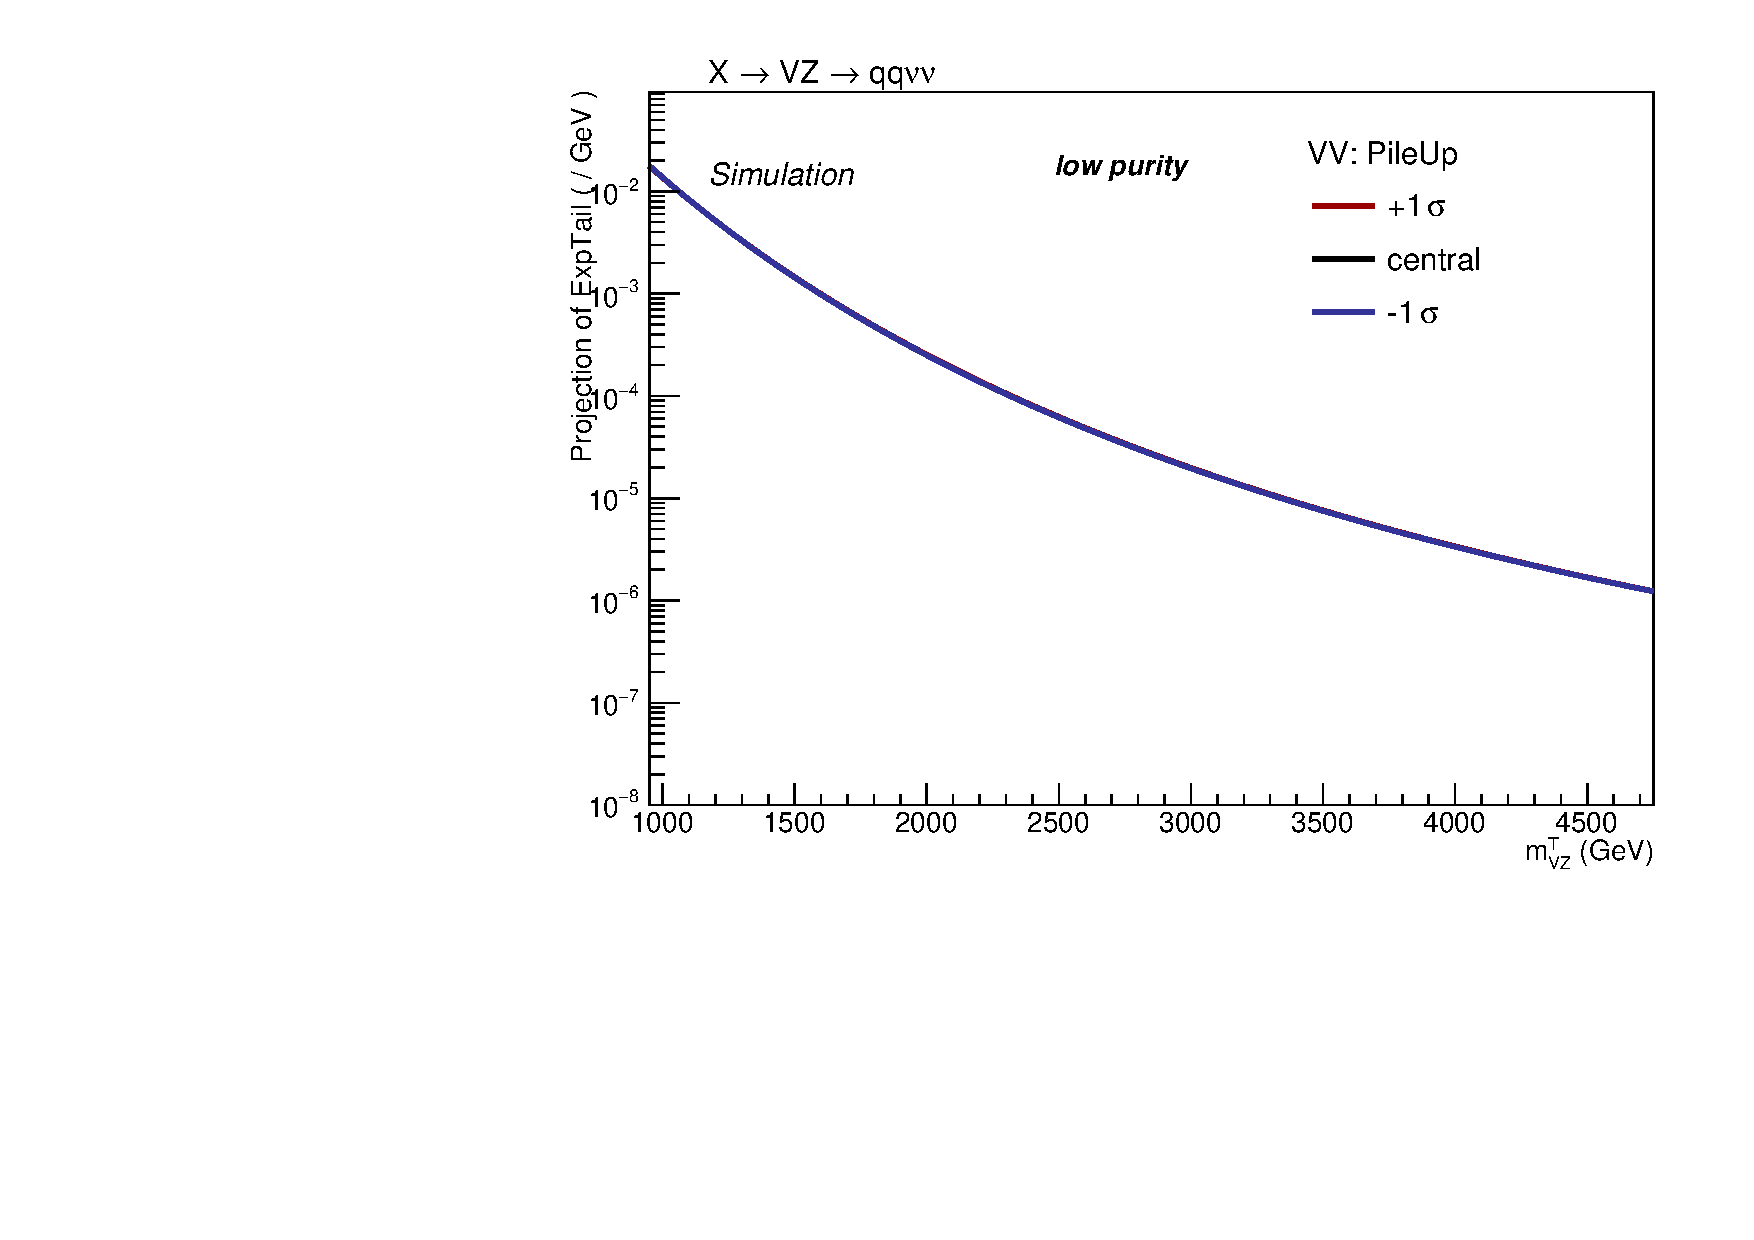
\includegraphics[width=.495\textwidth]{plotsAlpha_tesi/XVZnnlp/SysVV_PileUp.pdf}
     \\
     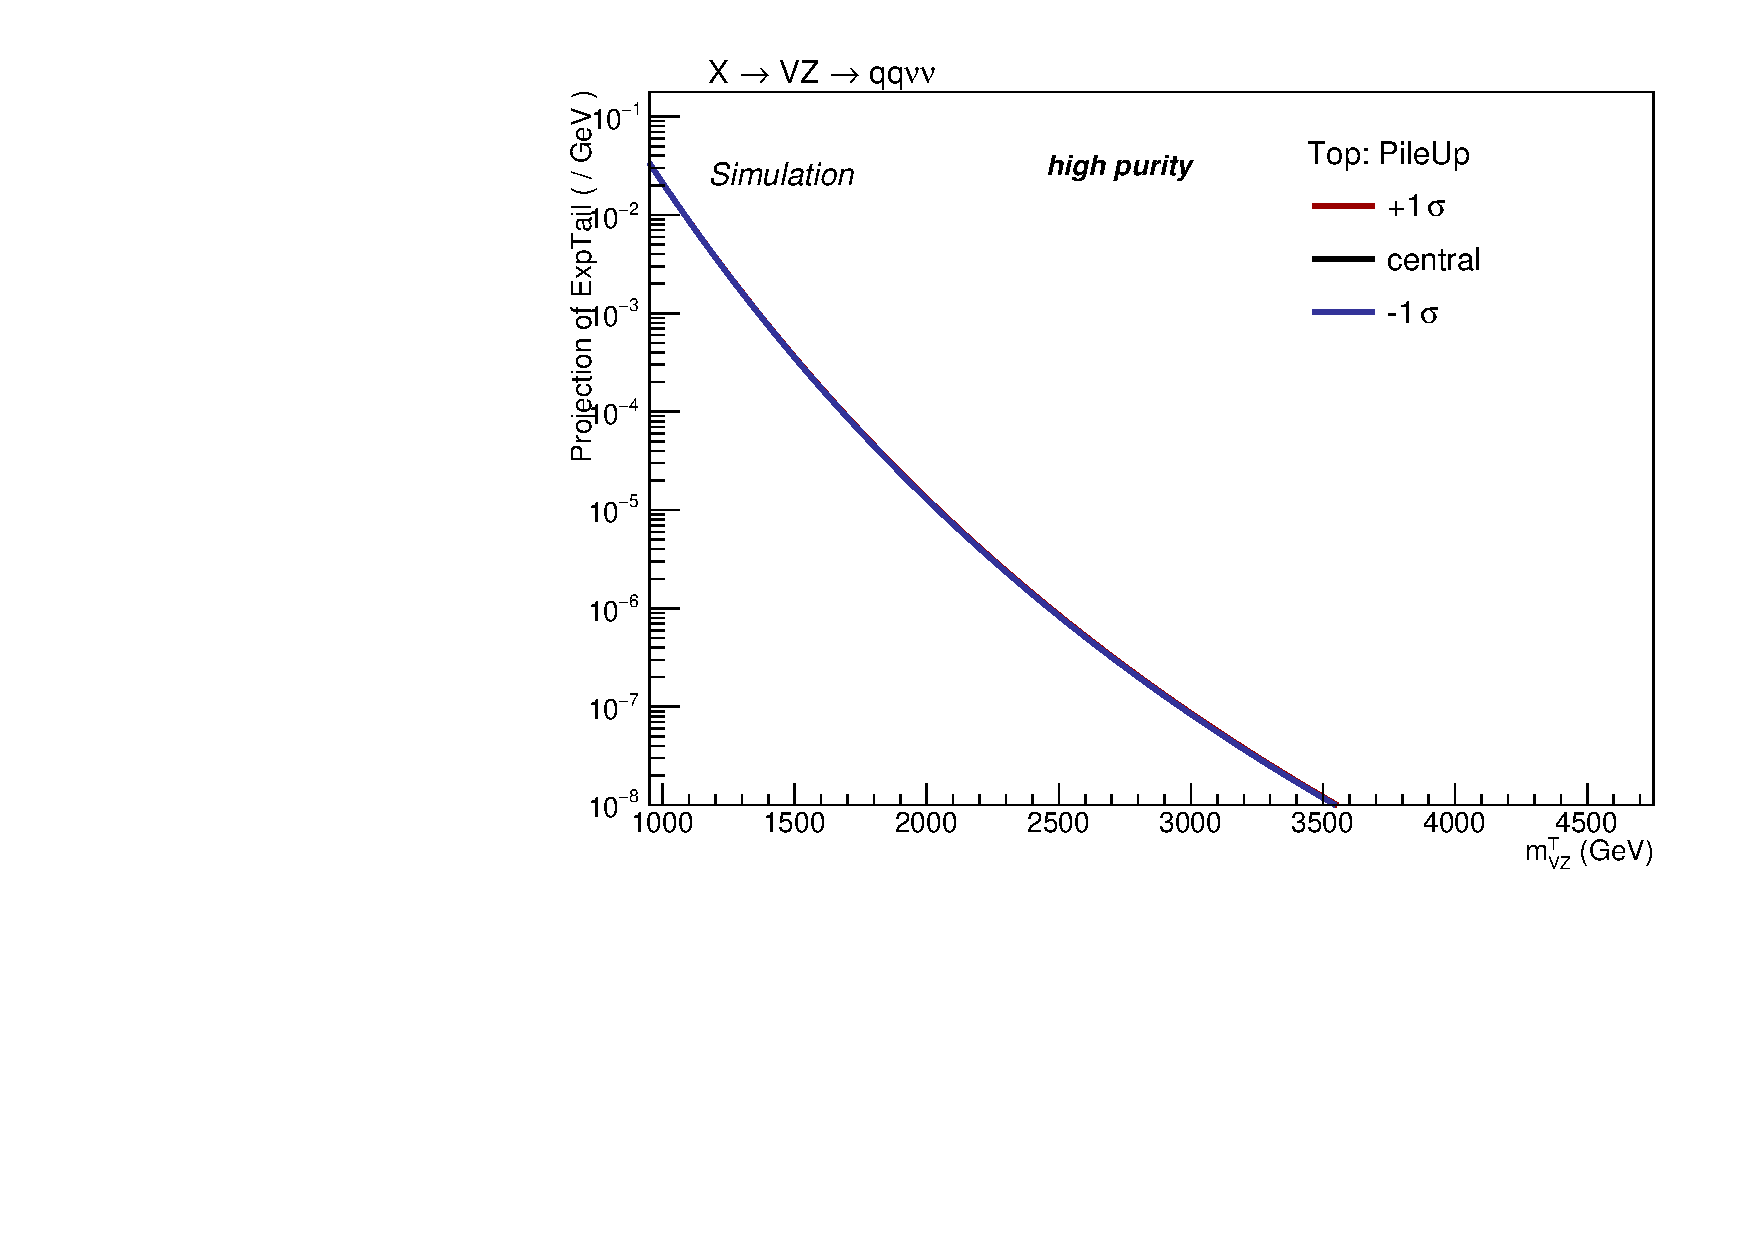
\includegraphics[width=.495\textwidth]{plotsAlpha_tesi/XVZnnhp/SysTop_PileUp.pdf}
     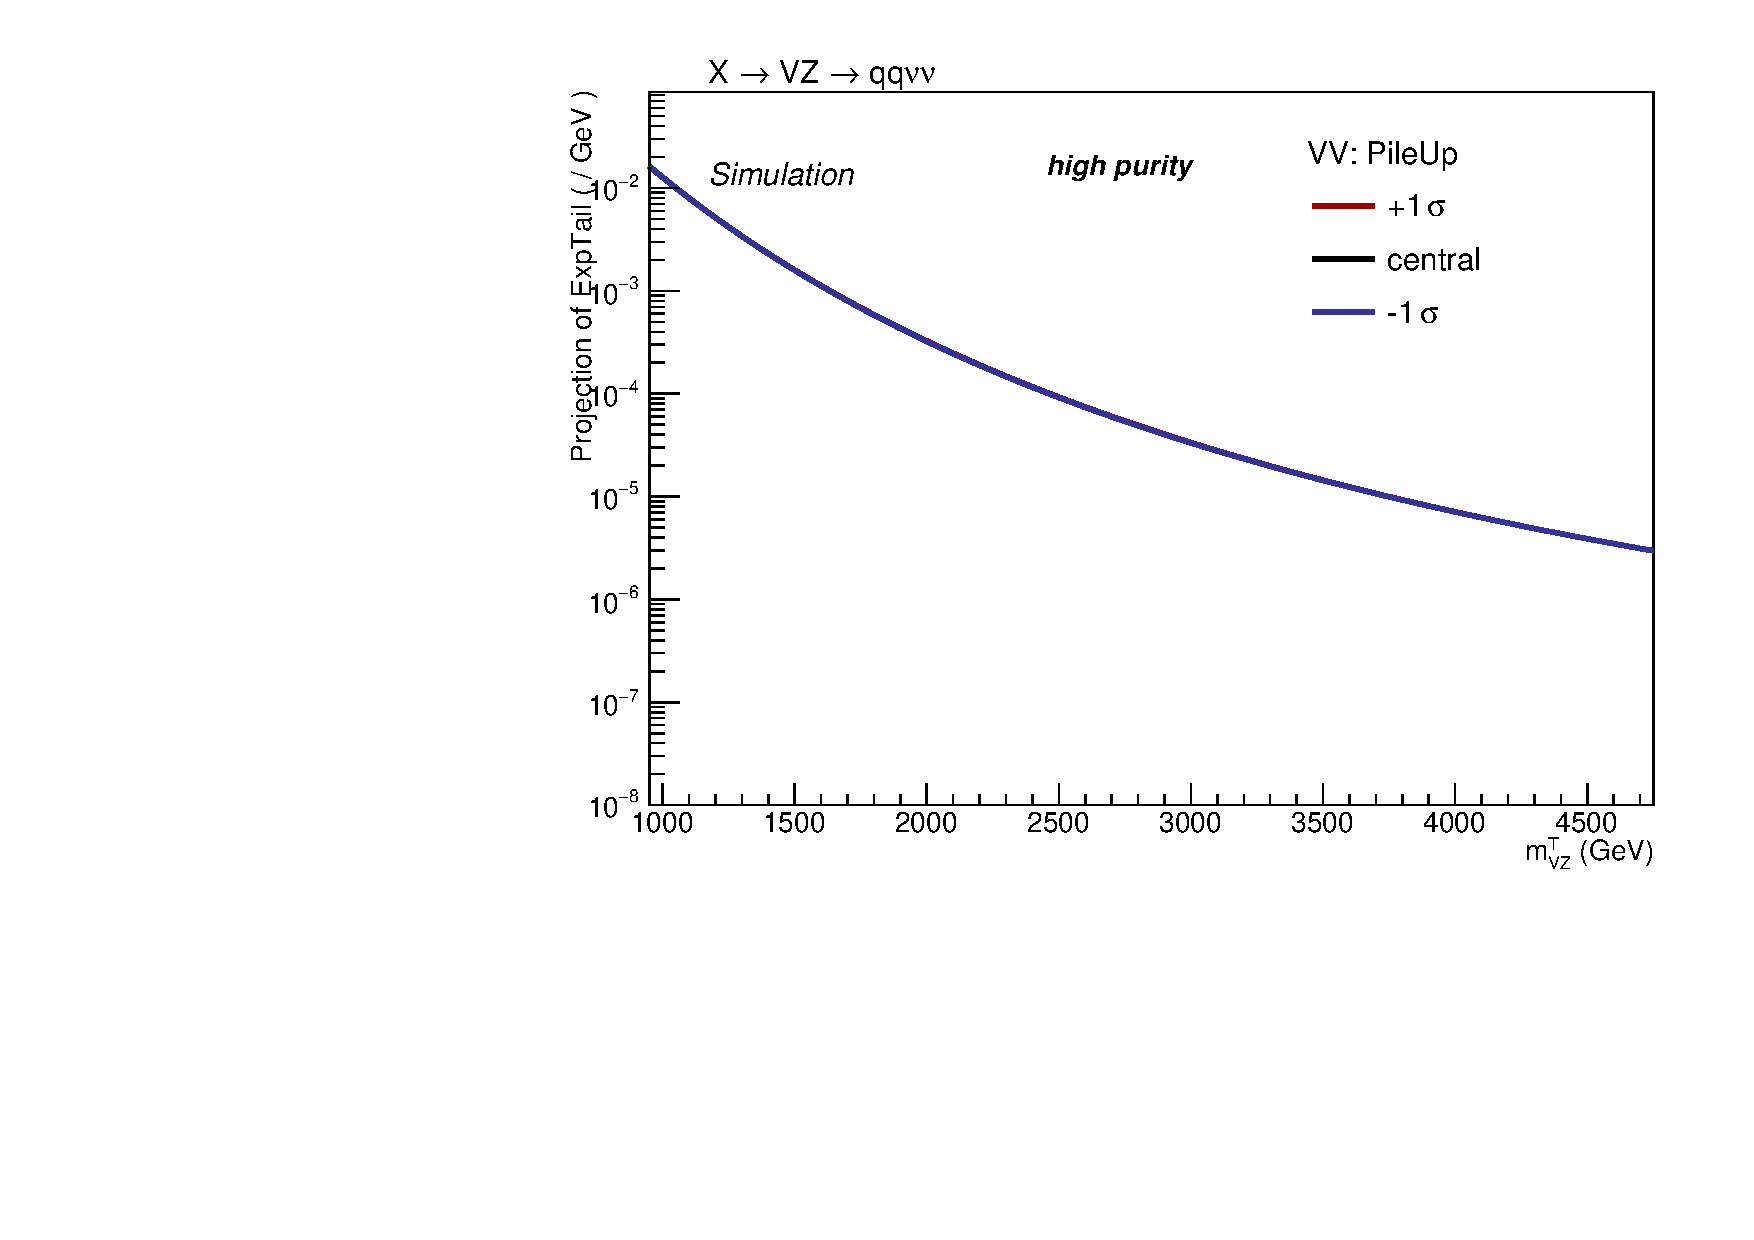
\includegraphics[width=.495\textwidth]{plotsAlpha_tesi/XVZnnhp/SysVV_PileUp.pdf}

   \end{center}
   \caption{Shape variations due to pile-up uncertainty obtained in the Top (left) and diboson (right) backgrounds, in the low-purity (top) and high-purity (bottom) category.}
   \label{fig:syspileup}
 \end{figure}


\subsubsection{QCD renormalization and factorization scale uncertainties}

Divergencies appearing in perturbative QCD calculation, used to predict the cross-sections and the spectra of the observables in Monte Carlo simulations, are absorbed in the renormalization and factorization scales, $\mu_R$ and $\mu_F$. Per-event weights are calculated for a variation of these scales by a factor 2. The two scales can be varied separately and independently, or together assuming 100\% correlation; the first approach is adopted. The weight is propagated up to the final distributions, accounting for normalization and shape uncertainties.

\noindent The QCD variations have negligible effect on signal acceptance and on the mean and sigma of the gaussian core of the Crystal Ball functions. The QCD factorization has an impact on top background shape (1.1\%) and normalization (3.1\%), and on diboson normalization (0.9\%). The QCD renormalization affects the top normalization (7.3\%) and diboson normalization (1.3\%).

 \begin{figure}[!htb]
   \begin{center}
     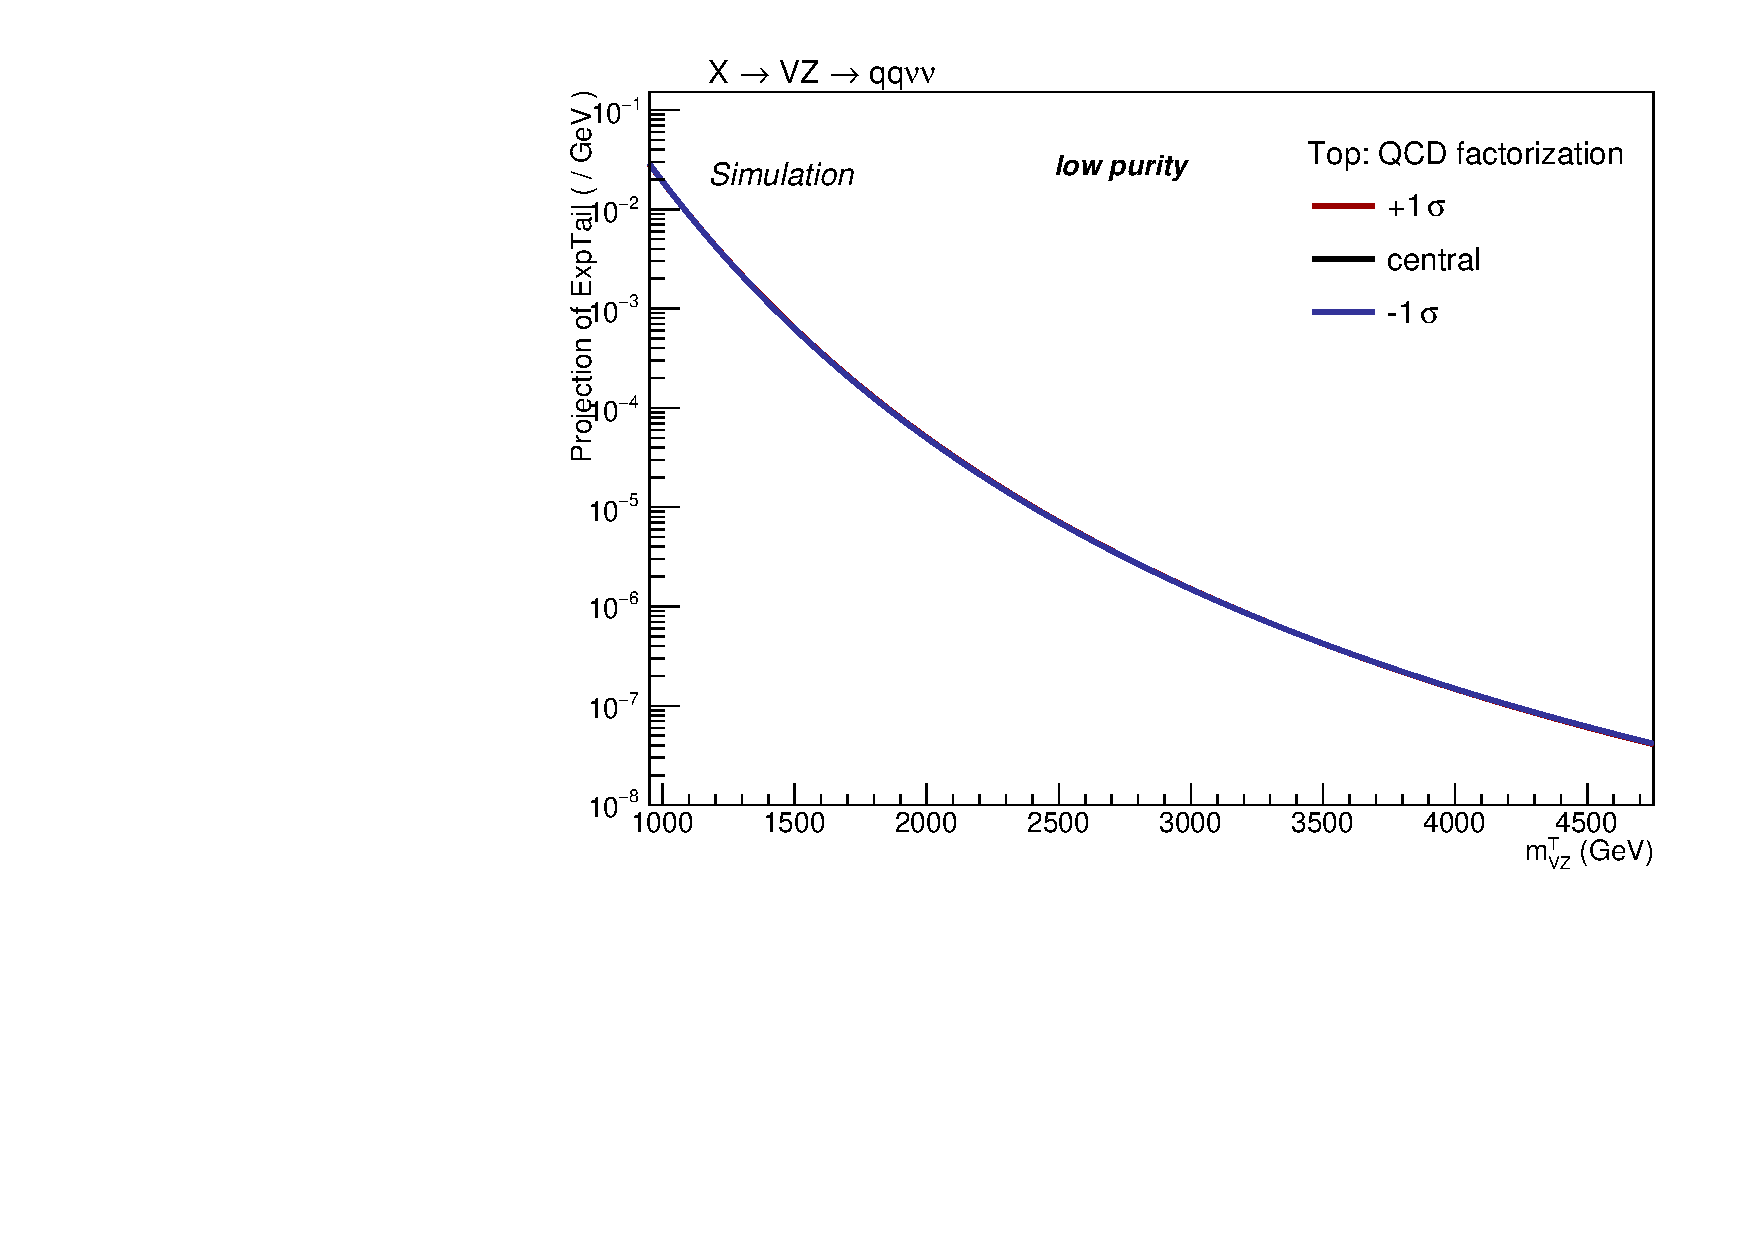
\includegraphics[width=.495\textwidth]{plotsAlpha_tesi/XVZnnlp/SysTop_QCD.pdf}
     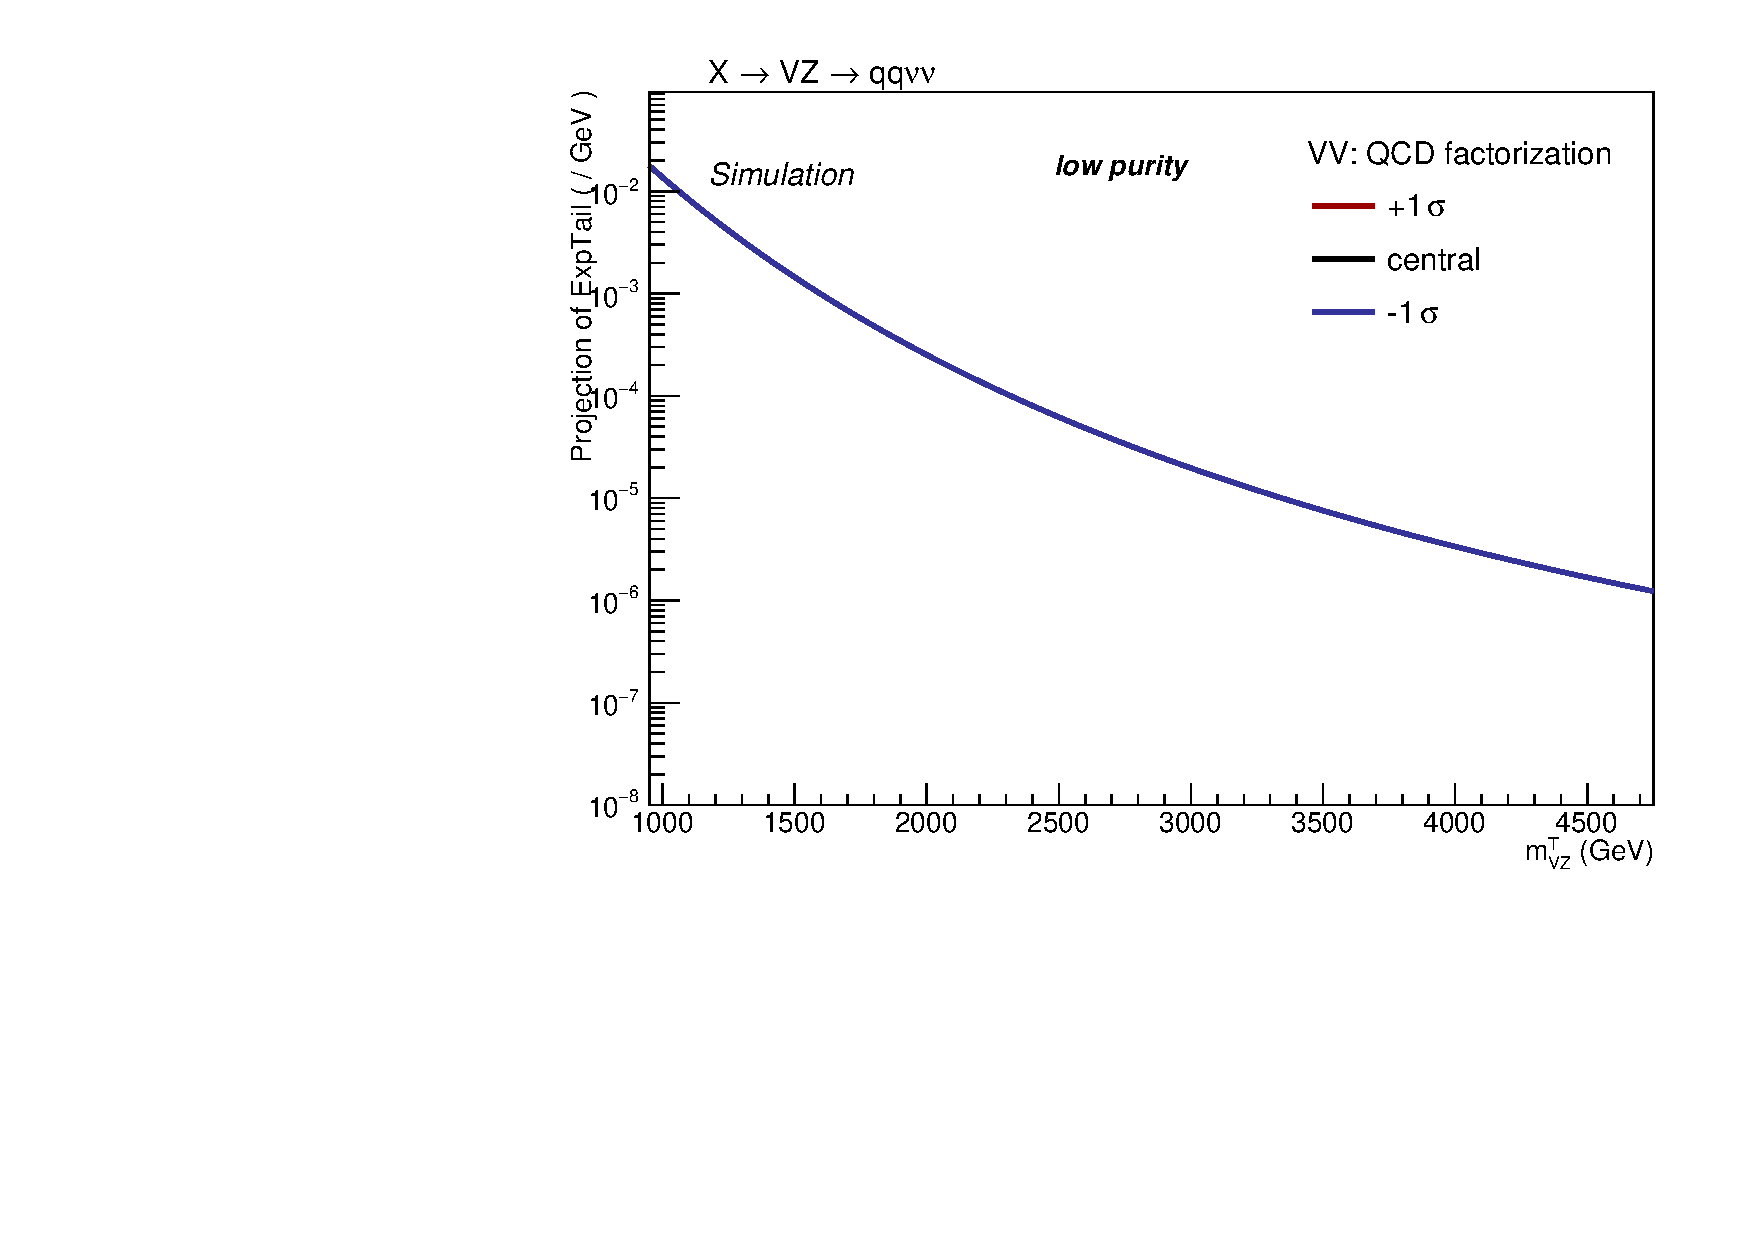
\includegraphics[width=.495\textwidth]{plotsAlpha_tesi/XVZnnlp/SysVV_QCD.pdf}
     \\
     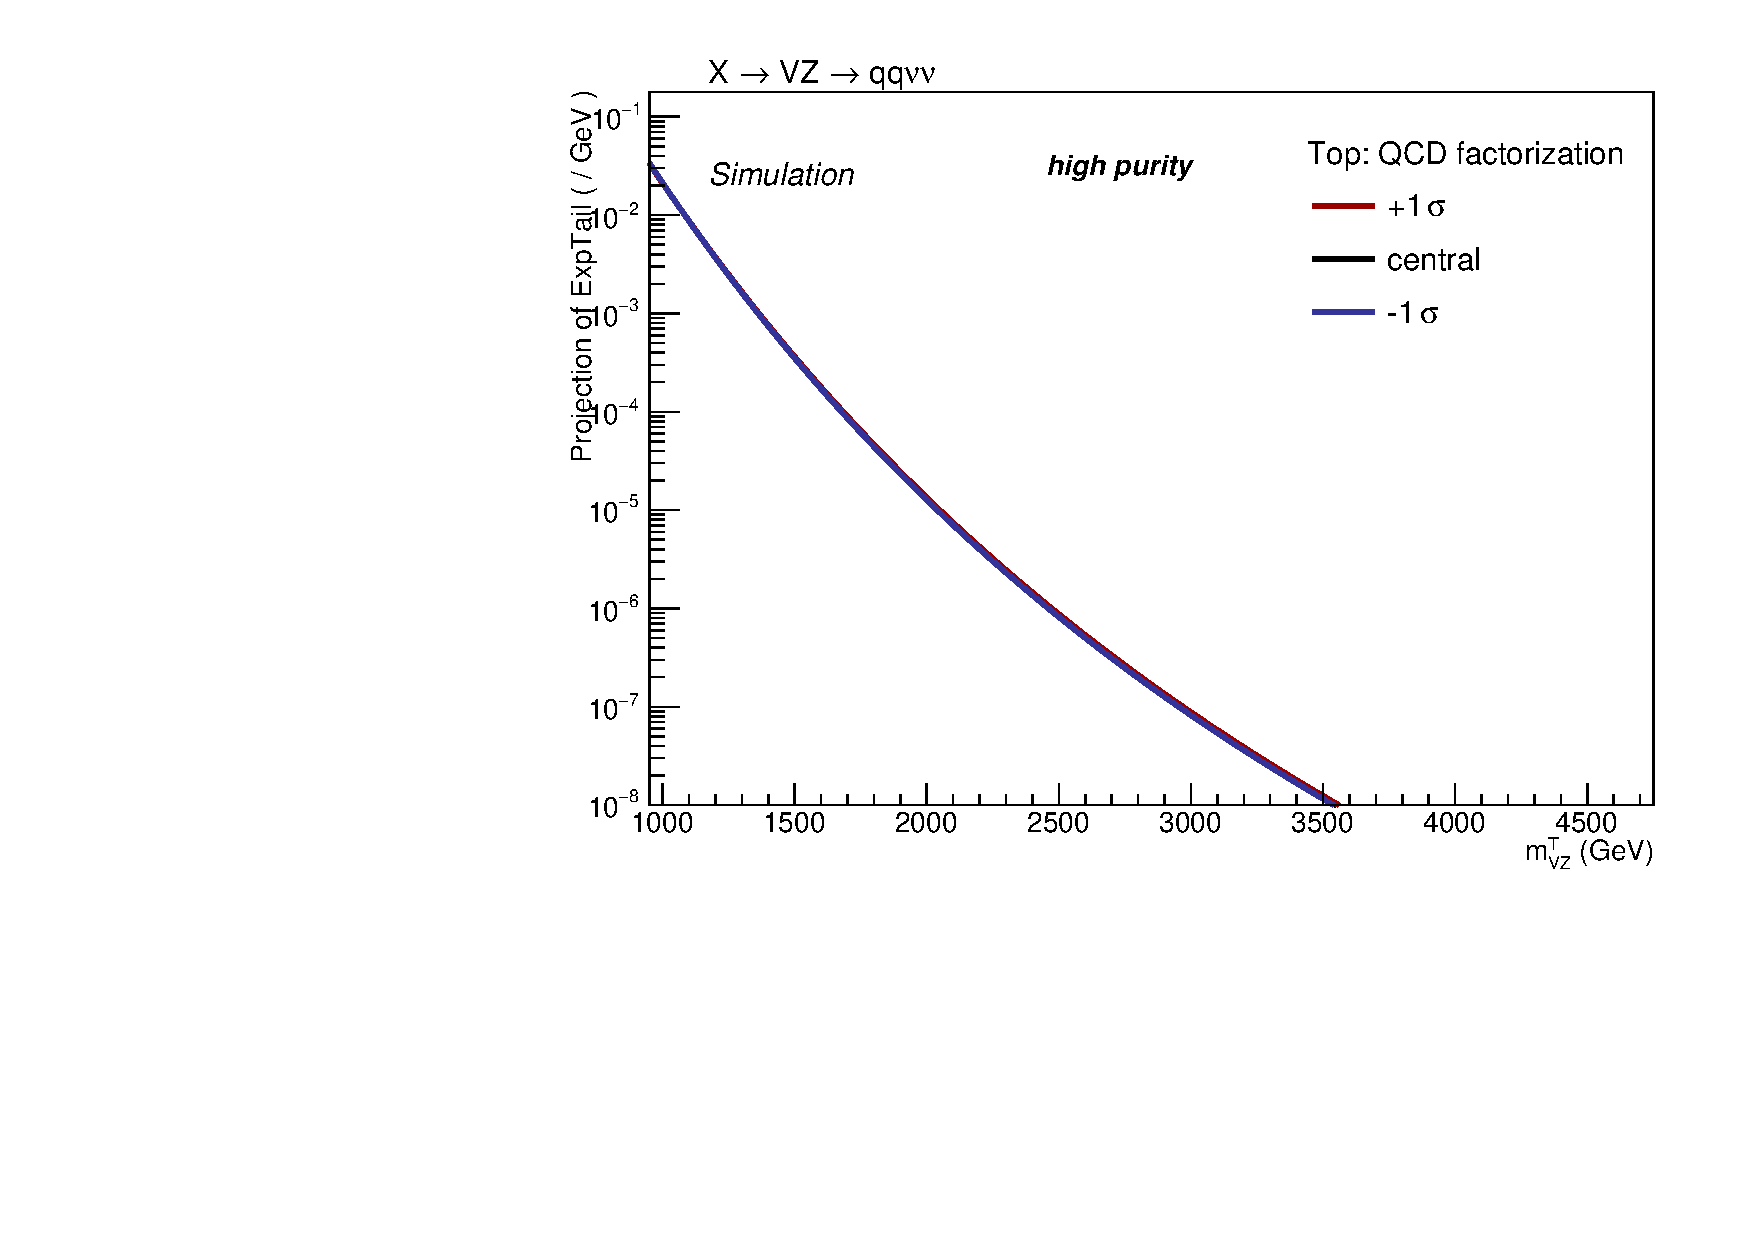
\includegraphics[width=.495\textwidth]{plotsAlpha_tesi/XVZnnhp/SysTop_QCD.pdf}
     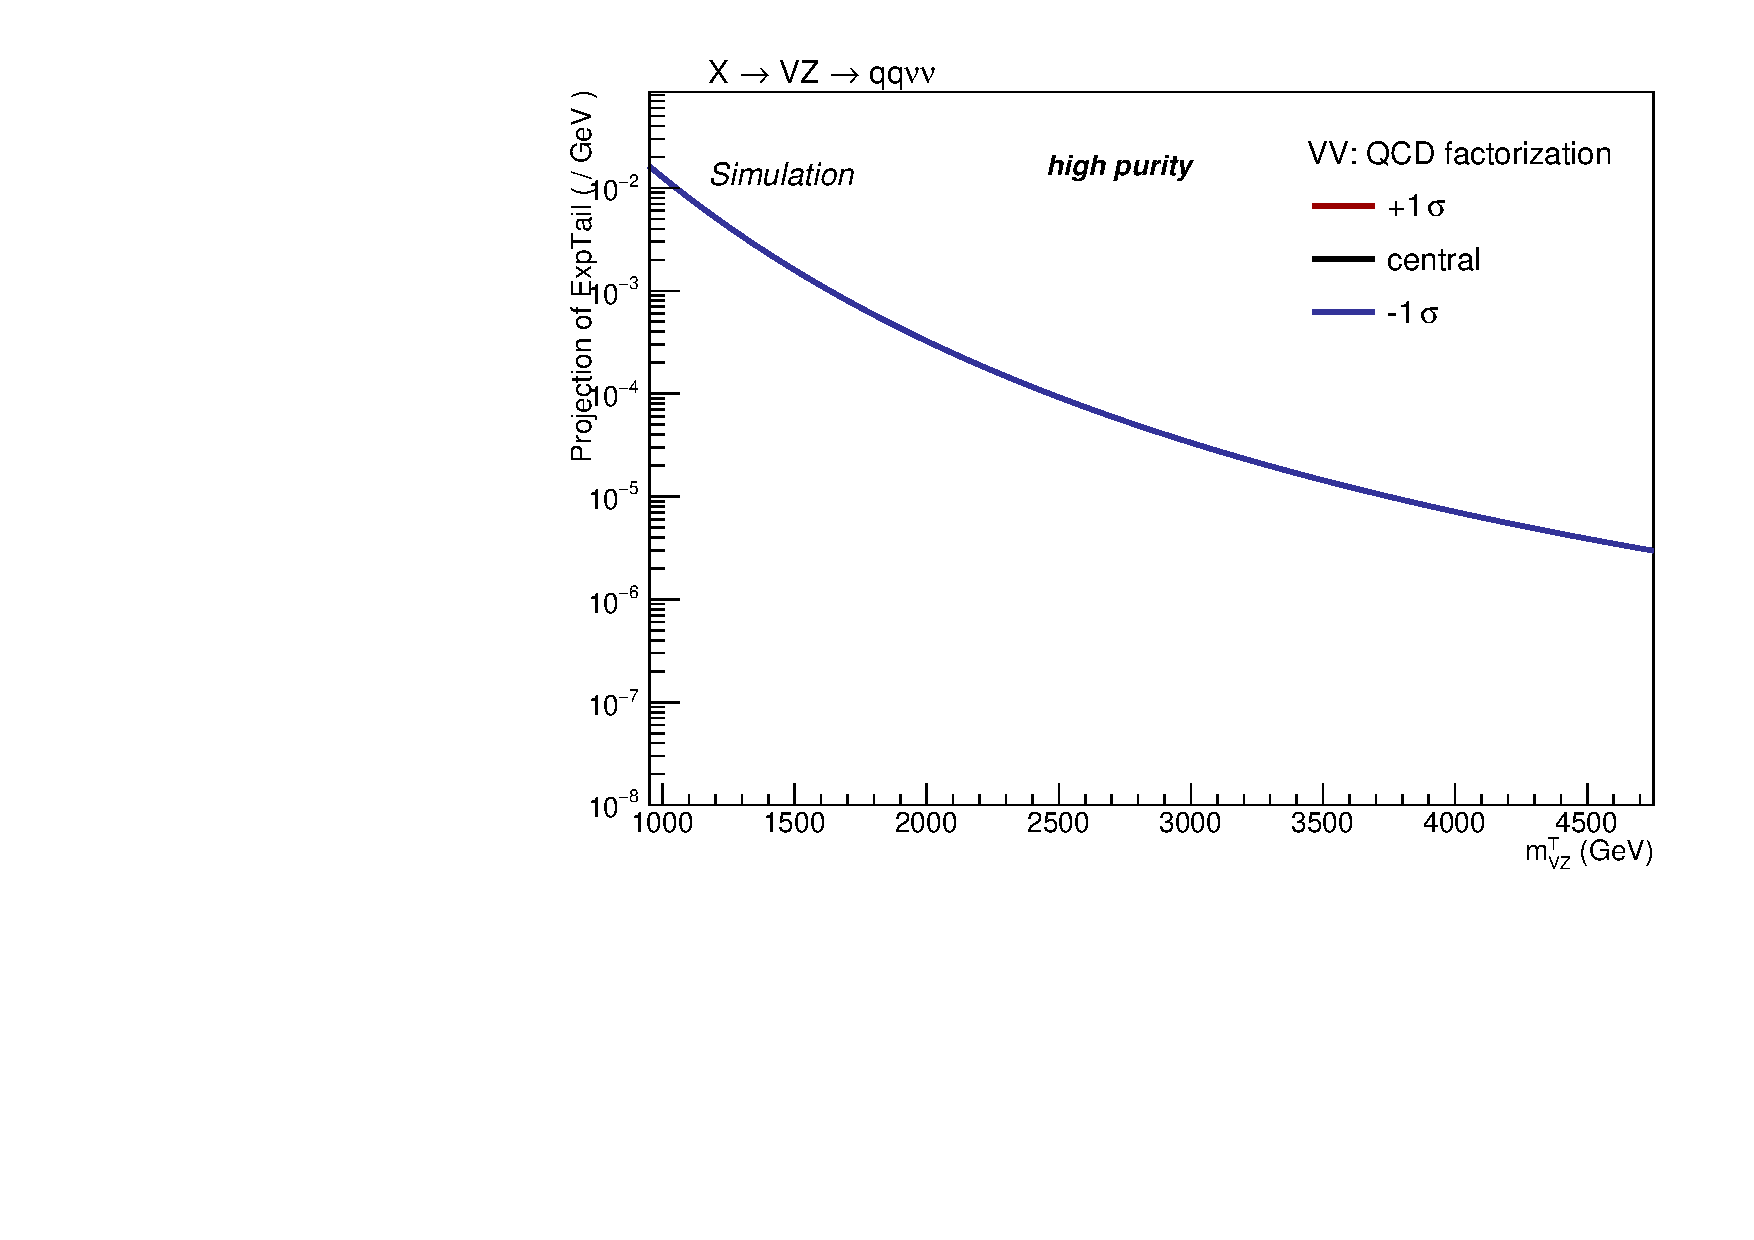
\includegraphics[width=.495\textwidth]{plotsAlpha_tesi/XVZnnhp/SysVV_QCD.pdf}

   \end{center}
   \caption{Shape variations due to QCD factorization in the Top (left) and diboson (right) backgrounds, in the low-purity (top) and high-purity (bottom) category.}
   \label{fig:sysScale}
 \end{figure}


\subsubsection{PDF}

Systematic uncertainties related to the PDFs parameters are estimated according to the PDF4LHC prescriptions~\cite{Butterworth:2015oua}, and using the NNPDF3.1~\cite{Ball:2017nwa} set. Each parameter describing the PDFs is varied within its uncertainty, resulting in a set of per-event weights. The 100 shifted weights have been considered together, by calculating the effect of their envelope, compared to their central values, on the expected event yield and on the \mtVZ distributions, and propagated as a normalization or shape uncertainty. The effect of the PDF uncertainty on the signal acceptance is found to be negligible, and it amounts to 10.3\% for top background normalization and 2.1\% for diboson background normalization. PDF uncertainties affect top background shape by 1.2\%.

 \begin{figure}[!htb]
   \begin{center}
     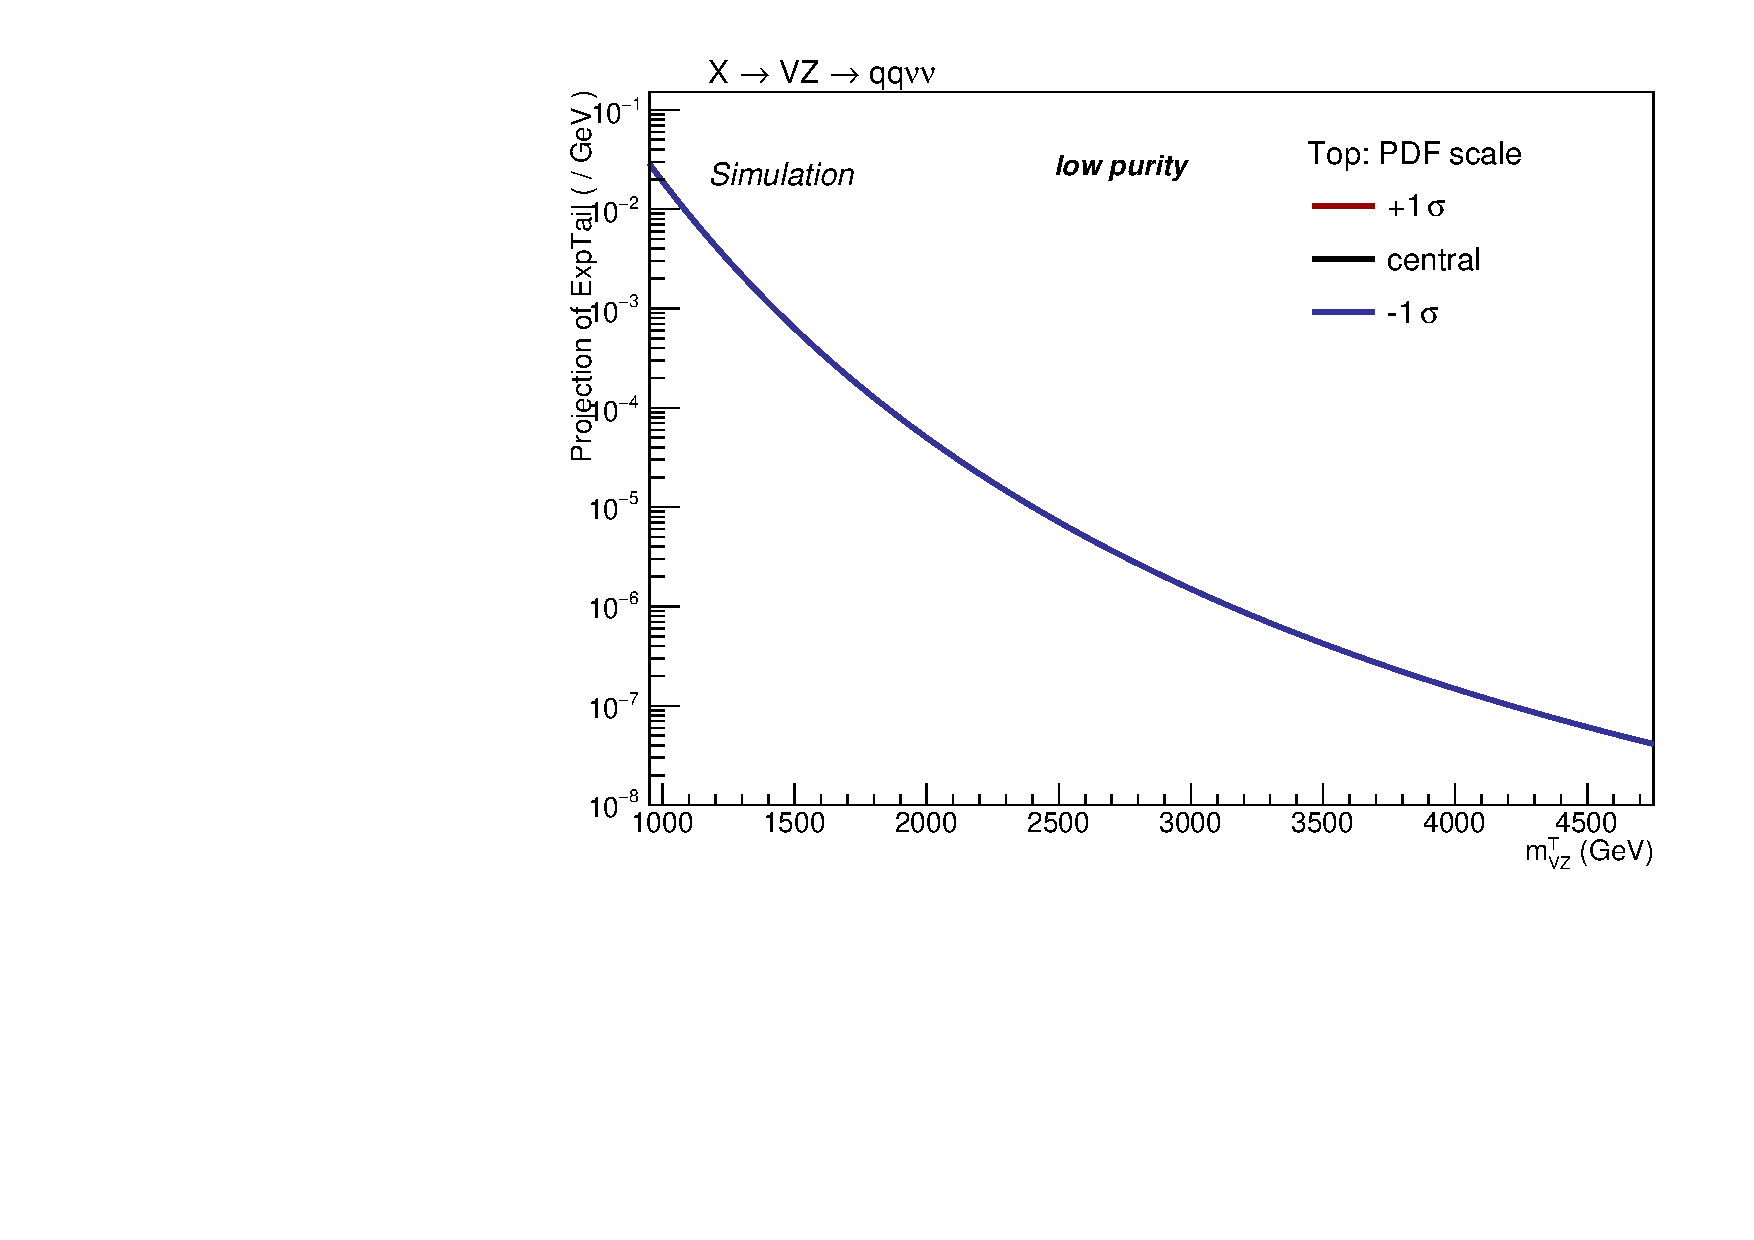
\includegraphics[width=.495\textwidth]{plotsAlpha_tesi/XVZnnlp/SysTop_Scale.pdf}
     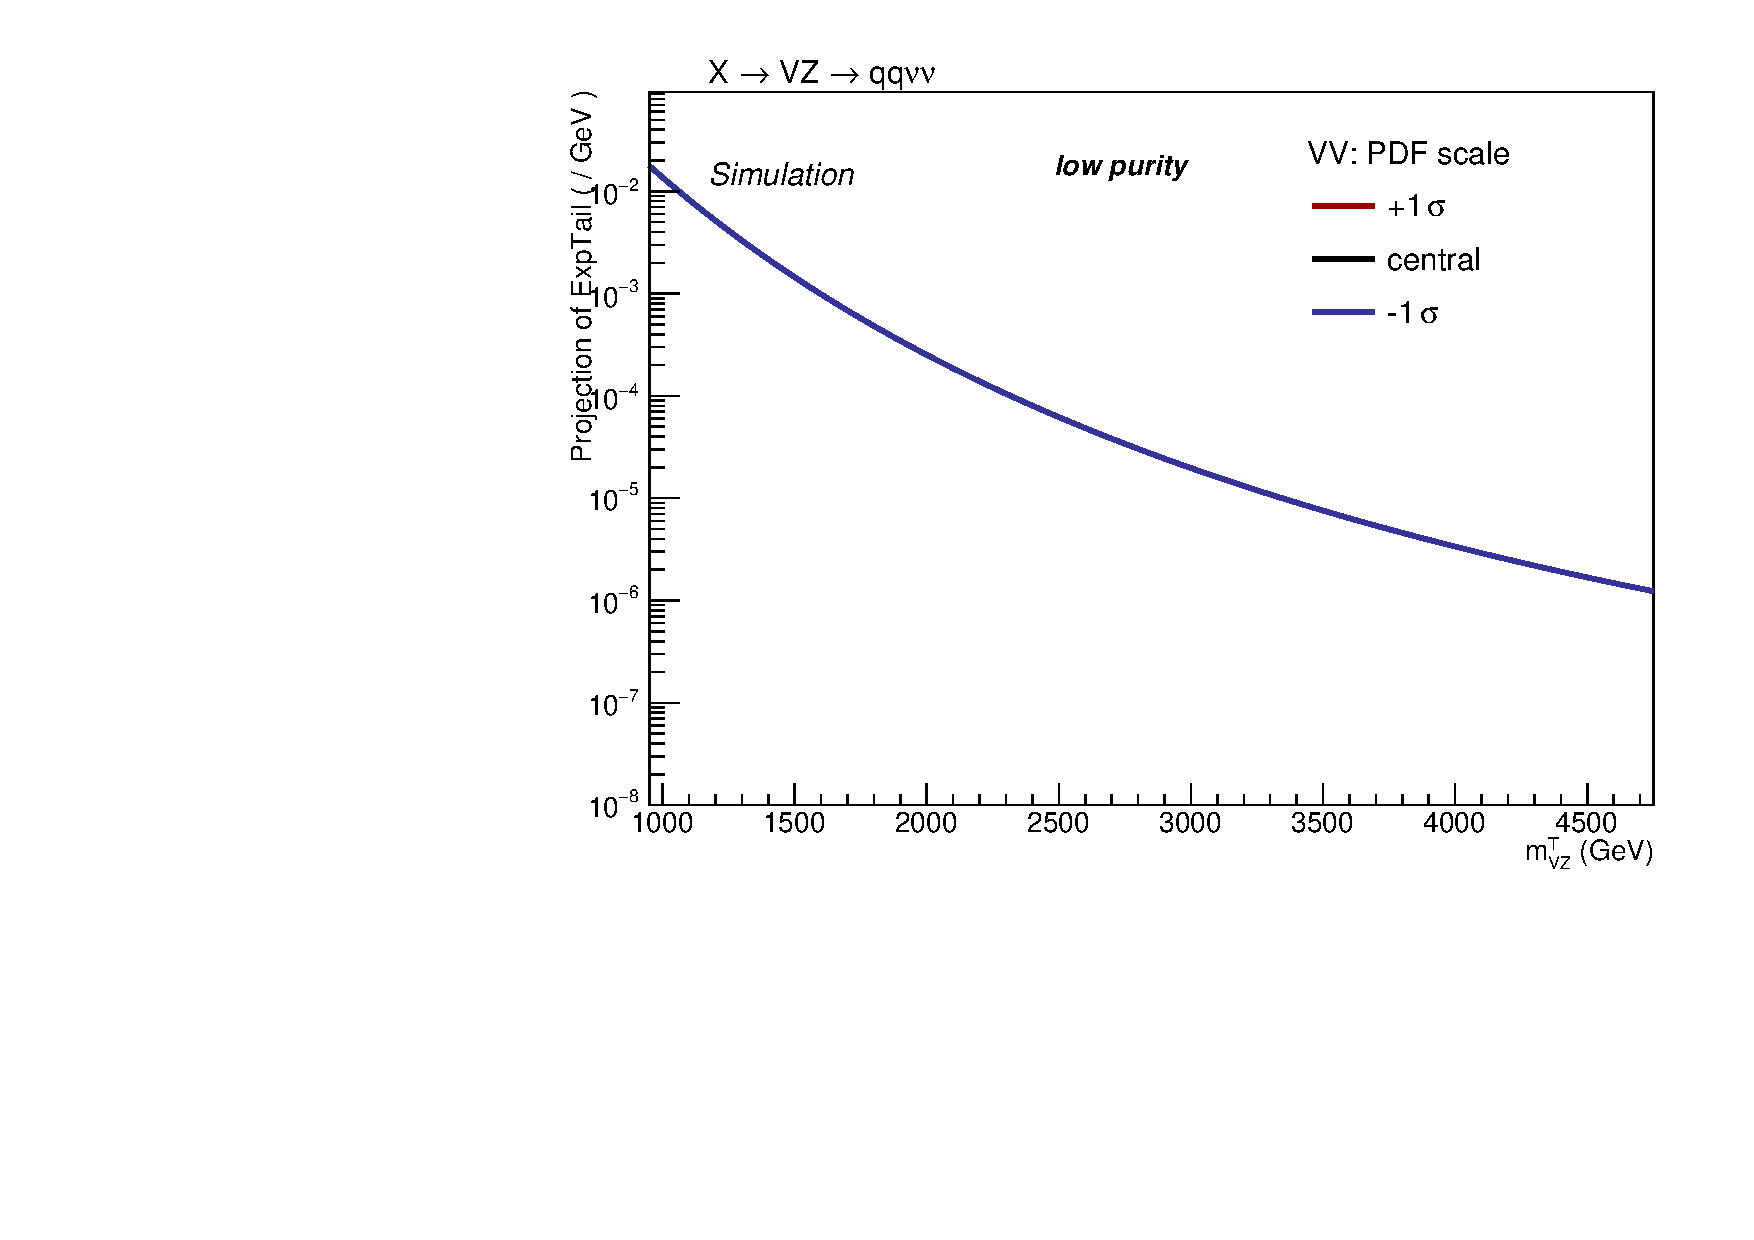
\includegraphics[width=.495\textwidth]{plotsAlpha_tesi/XVZnnlp/SysVV_Scale.pdf}
     \\
     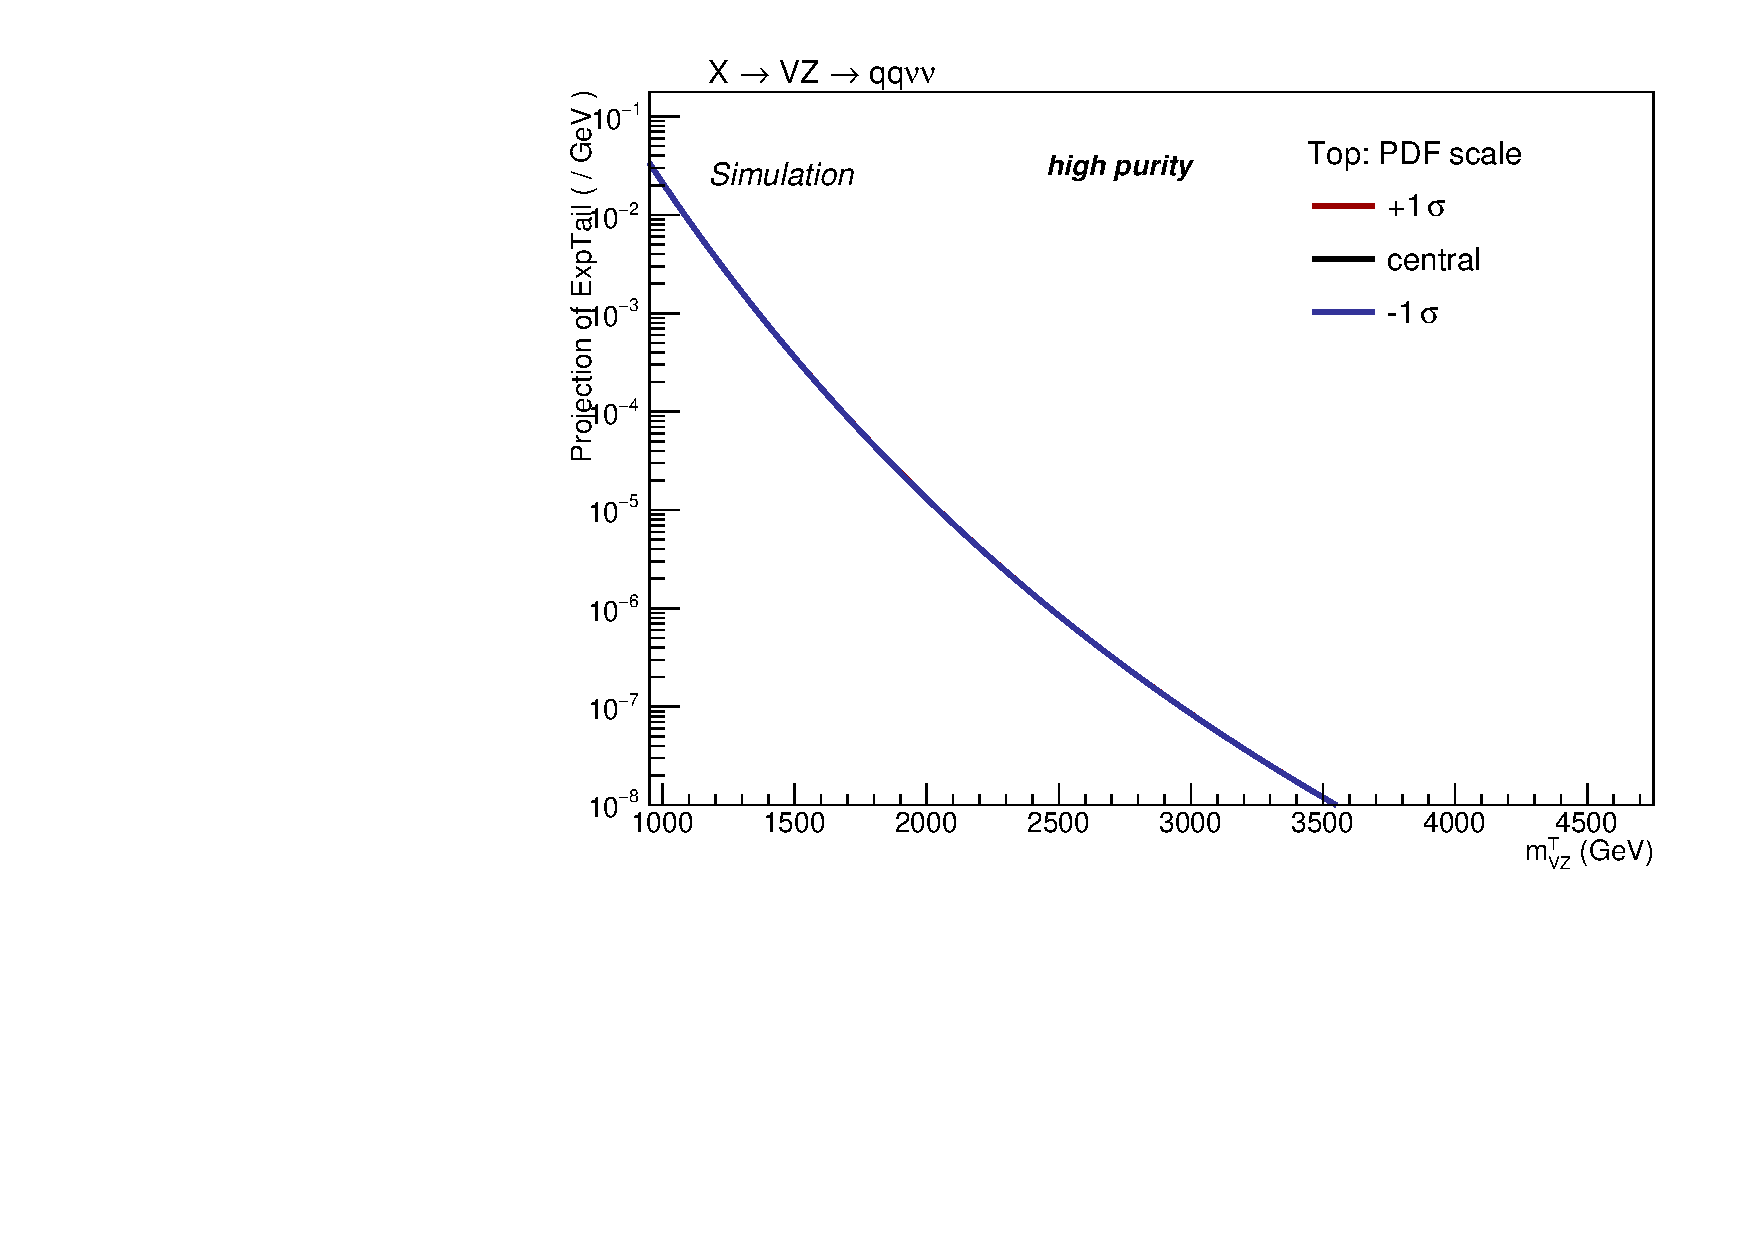
\includegraphics[width=.495\textwidth]{plotsAlpha_tesi/XVZnnhp/SysTop_Scale.pdf}
     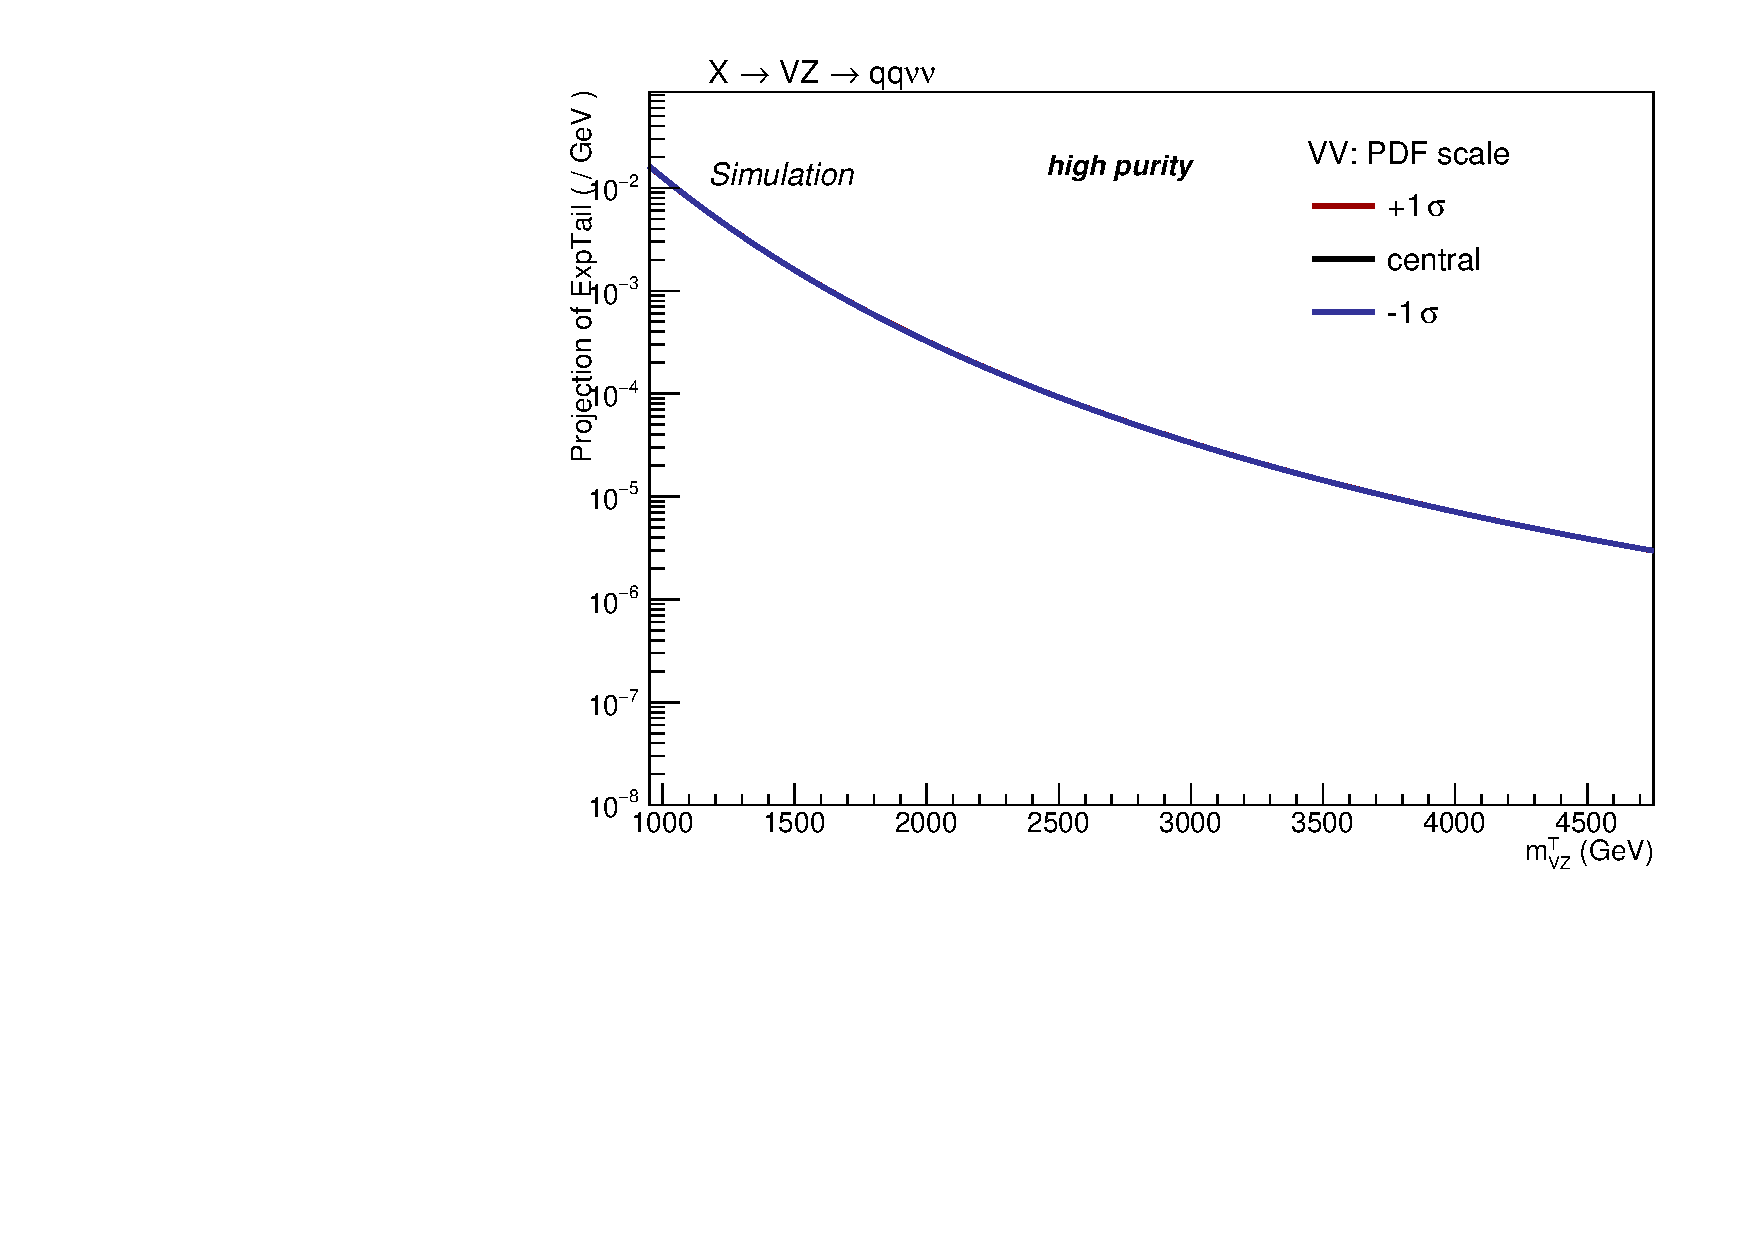
\includegraphics[width=.495\textwidth]{plotsAlpha_tesi/XVZnnhp/SysVV_Scale.pdf}

   \end{center}
   \caption{Shape variations due to PDF scale in the Top (left) and diboson (right) backgrounds, in the low-purity (top) and high-purity (bottom) category.}
   \label{fig:sysPDF}
 \end{figure}


\subsection{Summary}

A summary of all the systematic uncertainties is listed in tab.~\ref{tab:Sys}. In addition to those described in the previous sections, an uncertainty of $10\%$ on top background normalization is assumed, that is the uncertainty on the top production cross-sections obtained from CMS measurements (sec.~\ref{ssec:backgrounds}), and an uncertainty of $15\%$ is assigned to the diboson background normalization, due to the uncertainty on the cross-section measurements performed by CMS. An additional $3\%$ covers the uncertainty related to the tau veto, and an uncertainty of $2.5\%$ is assigned to the data integrated luminosity~\cite{CMS:2017sdi}.

%[FIXME: TO BE UPDATED WITH THE FINALIZED NUMBERS]

\begin{table}[!htb]
  \centering
  \caption{Summary of the systematic uncertainties for the backgrounds and signal samples. LP and HP indicate the uncertainty assigned for each purity category, low- and high-purity, respectively.}
  \label{tab:Sys}
  \begin{tabular}{l|ccccc}
                           & shape      & \V + jets & Top   & \VV    & Signal \\
    \hline
    \hline
    $\alpha$-function      & \checkmark & \checkmark   & - & - & - \\
    Bkg. normalization     &            & 4.8\%(LP)    & 68.2\%(LP) & 11.4\%(LP) & - \\
    (fit)                  &            & 14.7\%(HP)   & 47.7\%(HP) & 19.1\%(HP) & - \\
    Bkg. normalization     &            & 4.9\%(LP)    & - & - & - \\
    (alternative function) &            & 4.4\%(HP)   & - & - & - \\
    jet energy scale       & -          & -    & 0.2\% & 0.1\% & $<$0.1\% \\
    jet energy resolution  & -          & -    & 0.3\% & $<$0.1\%     & $<$0.1\% \\
    unclustered energy     & -          & -    & $<$0.1\%  & $<$0.1\% & $<$0.1\% \\
    jet mass scale         & \checkmark & -    & 0.7\% & 0.1\% & 1.8\% \\
    jet mass resolution    & \checkmark & -    & 3.1\% & 2.0\% & 5.1\% \\
    trigger                & -          & -    & 1.0\% & 0.9\% & 0.7-0.5\% \\
    \V boson tagging ($\tau_{21}$)  & - & -    & \multicolumn{3}{c}{11\% (HP), 23\% (LP)}  \\
    \V tagging extrapolation & -        & -    & 1.4\% (LP) & 1.7\% (LP) & 3.2-9.4\% (LP) \\
                           & -        & -    & 2.8\% (HP) & 3.3\% (HP) & 6.9-20.6\% (HP) \\
    b-tag veto             & -          & -    & 2.2\% & 0.3\% & 0.7-1.0\% \\
    pile-up                & \checkmark & -    & 0.3\% & 0.2\% & 0.4-0.7\% \\
    QCD renormalization    & \checkmark & -    & 7.3\% & 1.3\% & $<$0.1\%\\
    QCD factorization      & \checkmark & -    & 3.1\% & 0.9\% & $<$0.1\% \\
    PDF                    & \checkmark & -    & 10.3\%& 2.1\% & 10.4-18.9\% (scale) \\
    luminosity             & -          & -    & 2.5\% & 2.5\% & 2.5\% \\
    cross section          & -          & -    & 10\% & 15\% & - \\
    tau veto               & -          & -    & 3\% & 3\% & 3\% \\
  \end{tabular}
\end{table}


\clearpage

